\documentclass[12pt]{article}

\usepackage{graphicx}
\usepackage{paralist}
\usepackage{listings}
\usepackage{booktabs}
\usepackage{hyperref}
\usepackage{subfig}
\usepackage{float}

\oddsidemargin 0mm
\evensidemargin 0mm
\textwidth 160mm
\textheight 200mm

\pagestyle {plain}
\pagenumbering{arabic}

\newcounter{stepnum}

\title{CS/SE 2XB3 Lab 3 Report}
\author{
  Wang, Mingzhe\\
  \texttt{wangm235@mcmaster.ca}
  \and
  Li, Xing\\
  \texttt{li64@mcmaster.ca}
  \and
  Moon, Hyosik\\
  \texttt{moonh8@mcmaster.ca}
  }
\date{\today}

\begin{document}

\maketitle

This report concludes the main observations that we found in this week's lab, with the analysis that we did for the experiments of each methods.

\section{In-Place Version}
In this part, \verb|quicksort_inplace()| is implemented in an in-place way. Experiments will be tested on this version of quicksort.

\subsection{Expected advantages}
Before testing, the expected advantages of \verb|quicksort_inplace()| over \verb|my_quicksort()| are listed below:
\begin{itemize}
\item \textbf{Lower Space complexity}\\ Because \verb|quicksort_inplace()| is an in-place version, i.e. it does not create copies of list, its space complexity is low. That means it can perform better in cases where the storage space is limited, e.g. cache and internal memory.
\item \textbf{Possible higher performance due to no initialization}\\ The version of \verb|quicksort_copy()| actually initialize two arrays, namely \verb|left| and \verb|right|, each time it is called. This behavior is possible to induce longer running time. While \verb|quicksort_recursive()| does not share the same feature \--- all instructions are in-place.
\end{itemize}

\subsection{Test Result}
After the expected advantages are denoted, the test on the performance of \verb|my_quicksort()| and  \verb|quicksort_inplace()| is run. All the details of this experiment can be found in the source code, while specially some of the settings are as the following:
\begin{itemize}
\item The method \verb|copy()| is used to guarantee two random lists with the same elements are generated each run, instead of the wrong scenario that one list only points to another list.
\item To reduce the interference from unrelated factors, for each given value of $n$, the test is run 10 times.
\item The range of the given $n$ is $[0, 100, 200, \ldots, 10000)$ to better present the performance of these two versions.
\end{itemize}
~\newline\noindent The results of this test are showed below.

\begin{figure}[hbt!]
    \centering
    \subfloat[Time complexity of two versions]{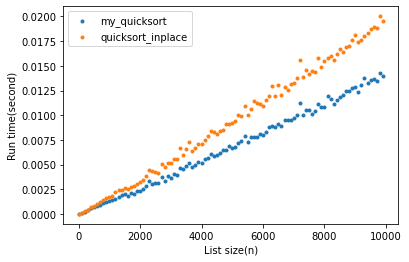
\includegraphics[width=0.5\textwidth]{Figures/my_vs_inp.png}\label{vs}}
    \hfill
    \subfloat[Percentage of how much faster]{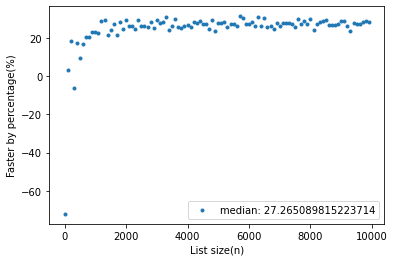
\includegraphics[width=0.4846\textwidth]{Figures/how_much.png}\label{how_much}}
    \caption{Test results}
\end{figure}

\newpage
\begin{itemize}
\item \textbf{Which implementation is better?}
From Figure \ref{vs}, it is apparent to determine that  \verb|my_quicksort()| actually performs better than \verb|quicksort_inplace()|.
\item \textbf{By how much?}
From Figure \ref{how_much}, the average percentage faster of \verb|my_quicksort()| against \verb|quicksort_inplace()| is approximately 27.265\%. It should be noted that the average percentage of faster tends to be stable after $n = 1000$.
\item \textbf{Which would you use in practice?}
Although we decide to use \verb|my_quicksort()| in the remainder of this lab because of its better performance, in practice, it is probably that the in-place version of quicksort will be preferred. This is because one of the advantages of quick sort is its locality, which makes quicksort usable in space limited cases like caches and internal memories. The performance loss of about 27\%, can be easily compensated by the high speed of cache access.

\end{itemize}


\section{Multi-Pivot}
In this part, multiple pivots are used rather than single pivot in the standard quick sort algorithm. The different experiments are made against the original sort function \verb|my_quicksort()| one by one, as requested by the lab specification. In order to compare apple-to-apple, we implement multi-pivot algorithm in the same style as \verb|my_quicksort()|.
(Figure \ref{Figure: mp_1}, \ref{Figure: mp_2}, \ref{Figure: mp_3})

~\newline\noindent Based on the graph below, the algorithm with single pivot always performs better on average, compared with dual-pivot, tri-pivot or quad-pivot. Therefore, it's recommended to use single-pivot-quick-sort as default in the remainder of this lab. 

~\newline\noindent In practice, multi-pivot algorithm may have its edge when the data set is huge and has to be handled in different computers with parallel computing, such as google searching with millions of computers all over the world. In that case, multi-pivot algorithm can group data by pivots and confine further sorting within a subarray with short physical distance. The performance could be dramatically better because no cross-subarray swap is needed in each sub-array, which normally comes with high cost due to internet communication.

\newpage

\begin{figure}[hbt!]
  \centering
  \subfloat[Dual Pivot vs Single Pivot]{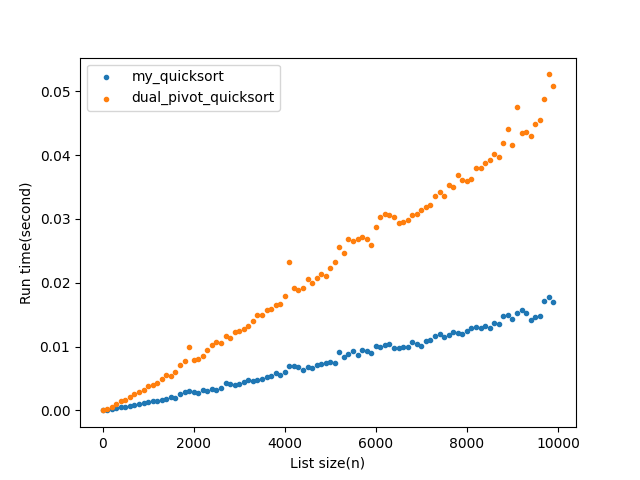
\includegraphics[width=0.5\textwidth]{Figures/multi_pivot_my_quicksort_dual_pivot_quicksort.png}\label{Figure: mp_1}}
  \subfloat[Tri Pivot vs Single Pivot]{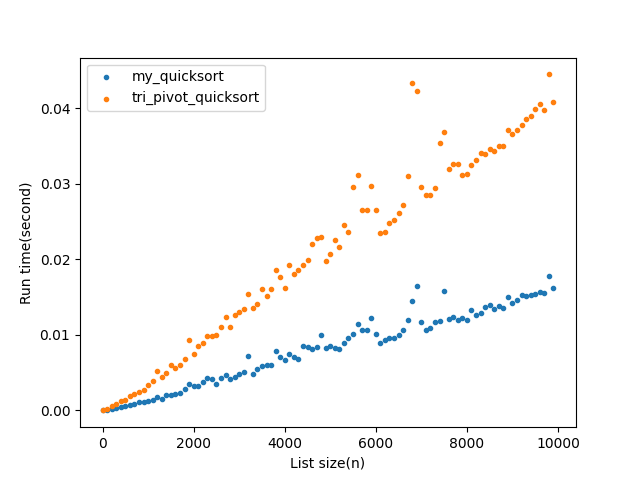
\includegraphics[width=0.5\textwidth]{Figures/multi_pivot_my_quicksort_tri_pivot_quicksort.png}\label{Figure: mp_2}}
  \hfill
  \subfloat[Quad Pivot vs Single Pivot]{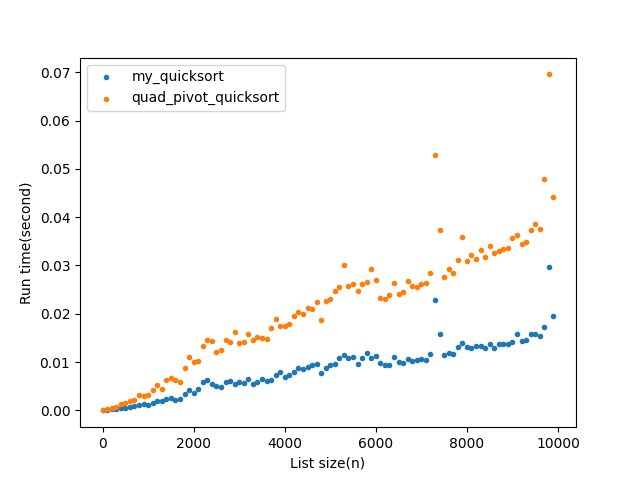
\includegraphics[width=0.5\textwidth]{Figures/multi_pivot_my_quicksort_quad_pivot_quicksort.png}\label{Figure: mp_3}}
  \caption{Test results}
\end{figure}

% \begin{figure}[h!]
% \centering
% 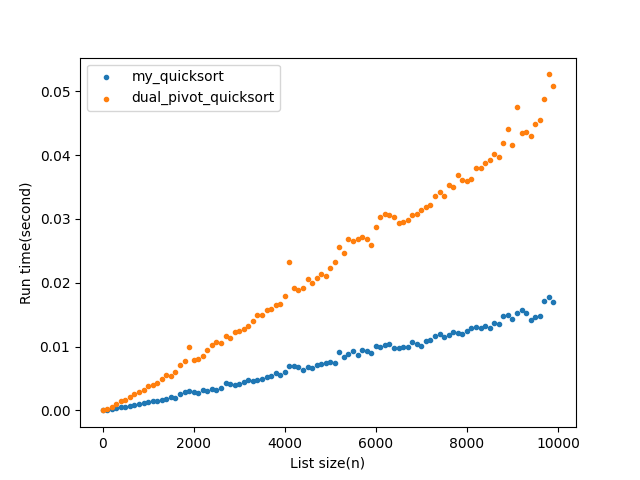
\includegraphics[width=0.6\textwidth,height=\textheight,keepaspectratio]{Figures/multi_pivot_my_quicksort_dual_pivot_quicksort.png}
% \caption{Dual Pivot vs Single Pivot}
% \label{Figure: mp_1}
% \end{figure}
% \begin{figure}[h!]
% \centering
% 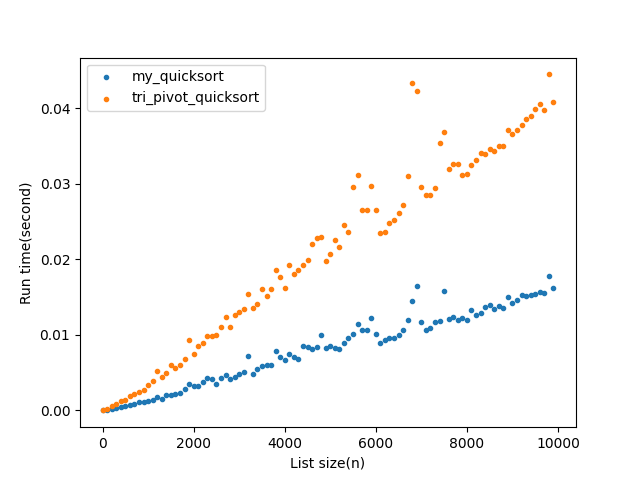
\includegraphics[width=0.6\textwidth,height=\textheight,keepaspectratio]{Figures/multi_pivot_my_quicksort_tri_pivot_quicksort.png}
% \caption{Tri Pivot vs Single Pivot}
% \label{Figure: mp_2}
% \end{figure}
% \begin{figure}[h!]
% \centering
% 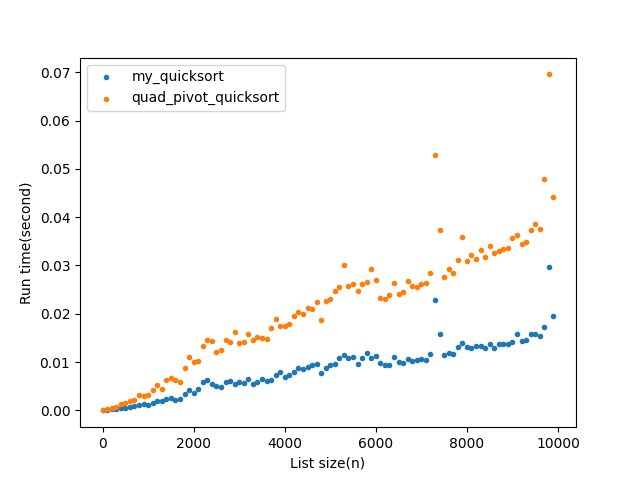
\includegraphics[width=0.6\textwidth,height=\textheight,keepaspectratio]{Figures/multi_pivot_my_quicksort_quad_pivot_quicksort.png}
% \caption{Quad Pivot vs Single Pivot}
% \label{Figure: mp_3}
% \end{figure}

\section{Worstcase Performance}
In this part, tests are set to evaluate the performance of quicksort in the worst cases.
\subsection{Quicksort average-case and worst-case}
Quicksort's worstcase happens when the elements are already sorted and the pivot is the first
or the last element. In this case, quicksort algorithm has the time complexity of 
$(n-1) + (n-2) \cdots + 1$, which means $\sum^{n-1}_{k=1}k \simeq O(n^{2})$. On the other hand,
when a list unsorted quicksort's average time complexity is $O(nlogn)$. We obtained the 
experimental values of the worst and average cases' time complexity (Figure \ref{qui.1}). 
In order to get the smooth graphs we ran the each point from
 5 to 50 times. As a result we were able to obtain the fact that the worst-case time complexity 
 is about $O(n^{2})$, and the average-case time complexity is close to $O(n)$. In order to
check more accurate time complexity of average-case, we tested it again by increasing 
the number of elements of the list to 10000. In the Figure \ref{qui.2}, 
we can surly see that the time complexity is about $O(nlogn)$.

\begin{figure}[hbt!]
    \centering
    \subfloat[Worst, Average cases $(n=1 \sim 1000)$]{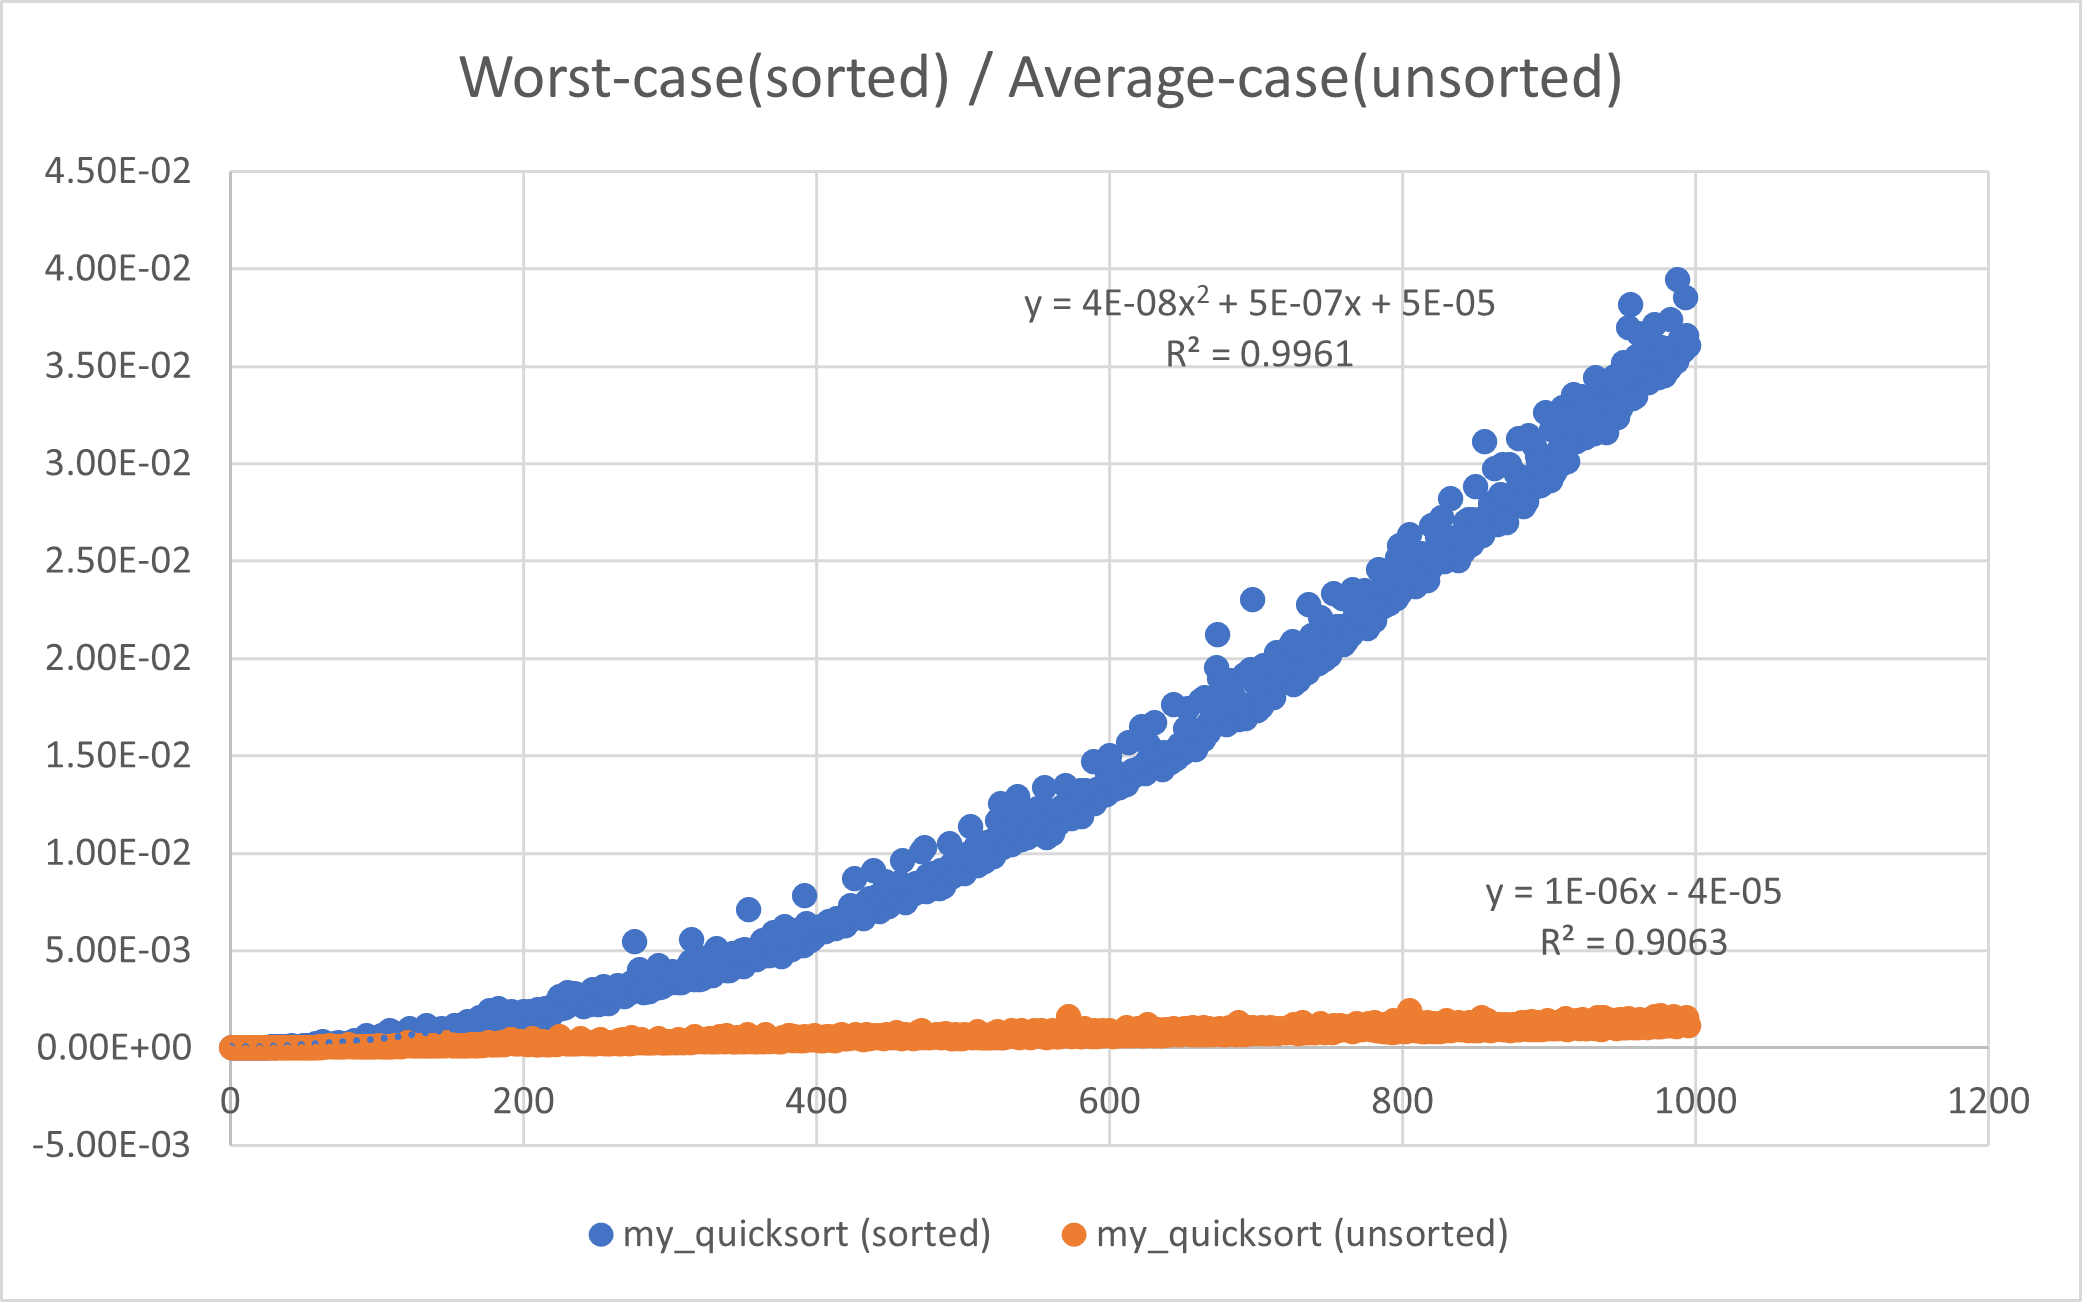
\includegraphics[width=0.49\textwidth]{Figures/quicksort1.png}\label{qui.1}}
    \hfill
    \subfloat[Average/n $(n=100 \sim 10000)$]{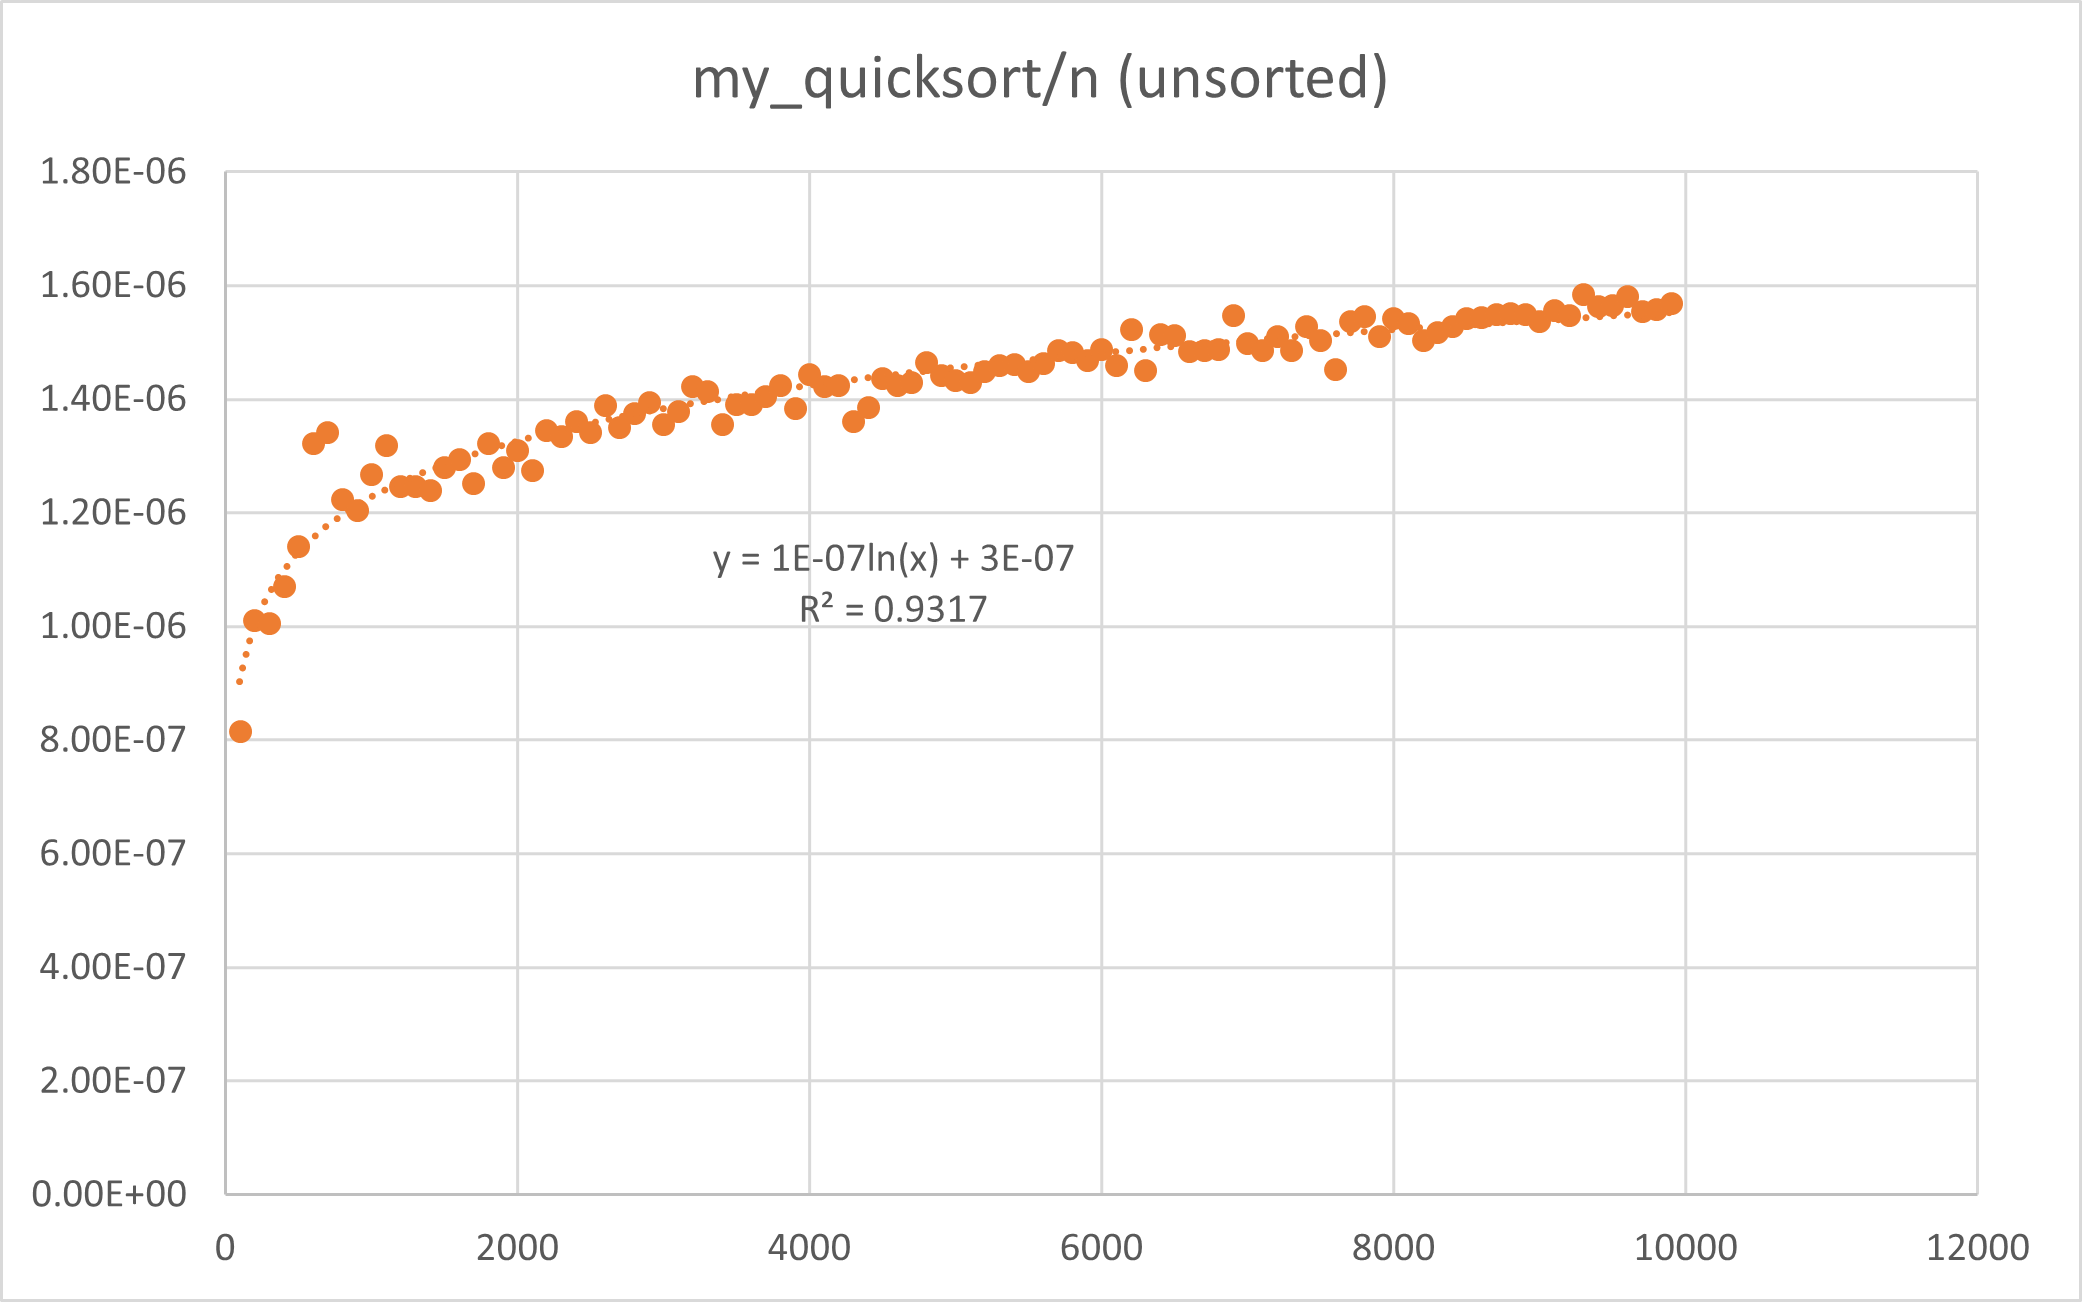
\includegraphics[width=0.49\textwidth]{Figures/quicksort2.png}\label{qui.2}}
    \caption{Time complexities of worst and average cases}
\end{figure}

\newpage
\subsection{Quicksort vs Elementary sorts ($n=1 \sim 1000$, $factor=0$, $0.01$)}
The second question was that among the optimized elementary sorting algorithms which one will
outpeform the quicksort algorithm for a nearly sorted list. We expected that bubble and insertion will 
outperform the quicksort implementation, because they will stop or minimise comparison when
a list is sorted. But the result was different. With the factor 0, which is totally sorted,
bubble and insertion sorts surpassed the quicksort (Figure \ref{sorted0}). But in the case of low factor,
which is 0.01, only insertion sort outperformed the quicksort (Figure \ref{sorted001}). This is because 
if there is at least one element which is not sorted in the list, bubble sort should continue
to sort the list to the end. Consequently, if a list isn't sorted totally, it doesn't
 reduce bubble sort's time complexity. However, with insertion sort, if a side of
 the list is sorted, then it doesn't need to go through the remaining part of the sorted list.    

\begin{figure}[hbt!]
  \centering
  \subfloat[$factor=0$, $n=1 \sim 1000$]{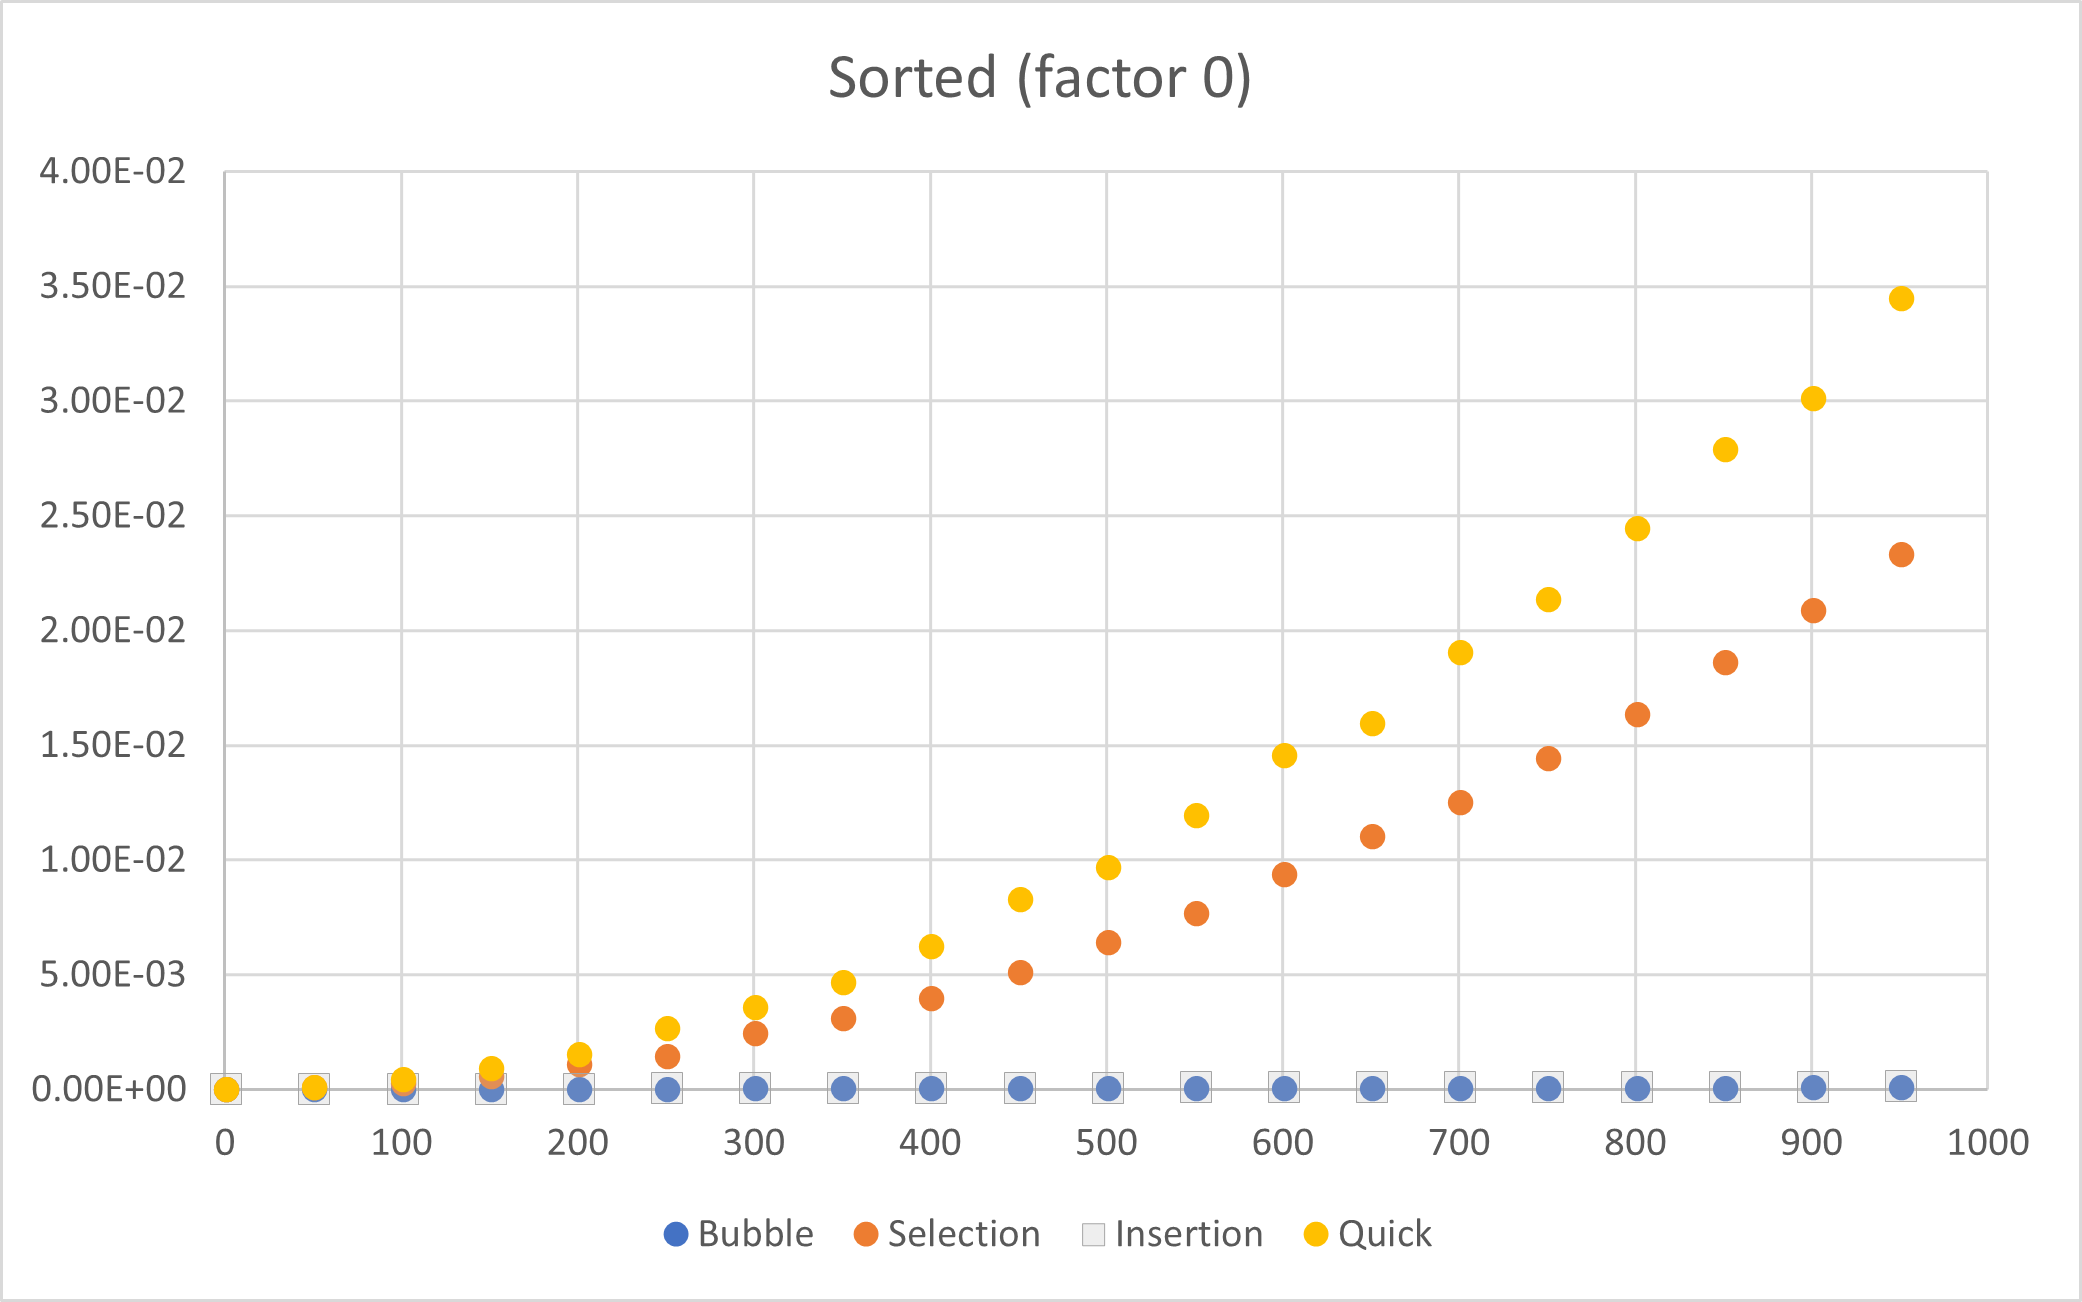
\includegraphics[width=0.49\textwidth]{Figures/sorted0.png}\label{sorted0}}
  \hfill
  \subfloat[$factor=0.01$, $n=1 \sim 1000$]{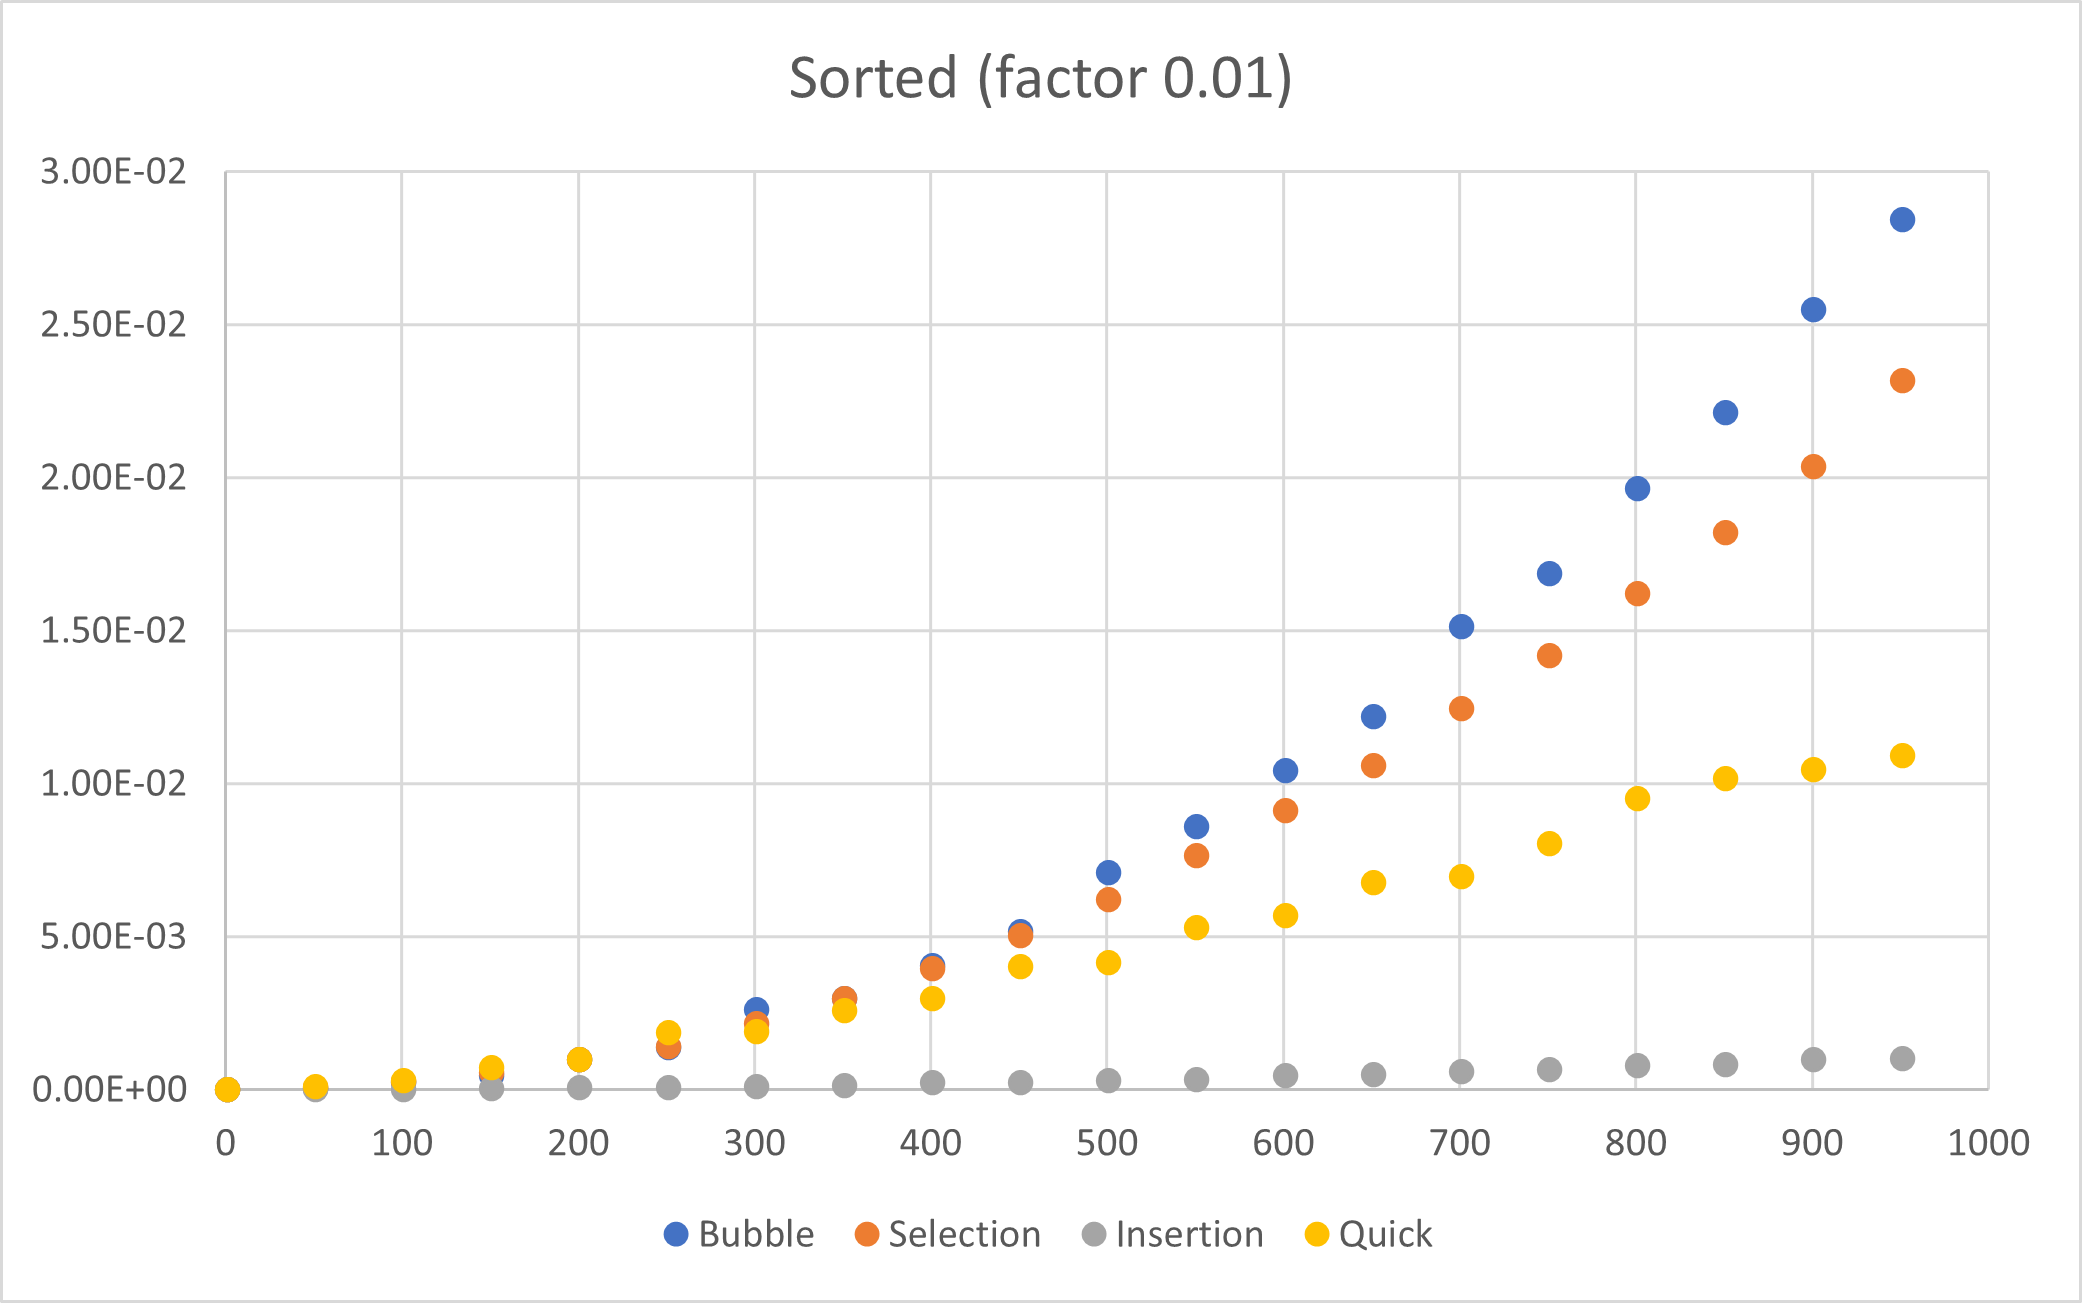
\includegraphics[width=0.49\textwidth]{Figures/sorted001.png}\label{sorted001}}
  \caption{Time complexities of sorting algorithms}
\end{figure}

\subsection{Quicksort vs Elementary sorts ($n=1000$, $factor=0.005 \sim  0.2$)}
This section compared quicksort and elementary sorts' performance based on a list of length 1000 
and near-sorted factors. The near-sorted factors change from 0.005 to 0.2, 
0.005 at a time. When the value becomes 0.045, quicksort outperforms the insertion sort 
(Figure \ref{sorted0005}). This result shows that if a length 1000's list is sorted more 
than $95.5\%$, then insertion sort's time performance is the best.   
We tested further to check that this fact can be applicable when the list's length 
is relatively small which is 100. As shown Figure \ref{sorted0005n100},
insertion sort is still the best. This is because when a list is nearly
sorted, insertion sort's time complexity is best which is close to $O(n)$, 
but quicksort's time complexity is worst which is close to $O(n^{2})$
 (Table \ref{time complexity}).

 \bigskip

 \begin{figure}[hbt!]
  \centering
  \subfloat[$factor=0.005 \sim  0.2$, $n=1000$]{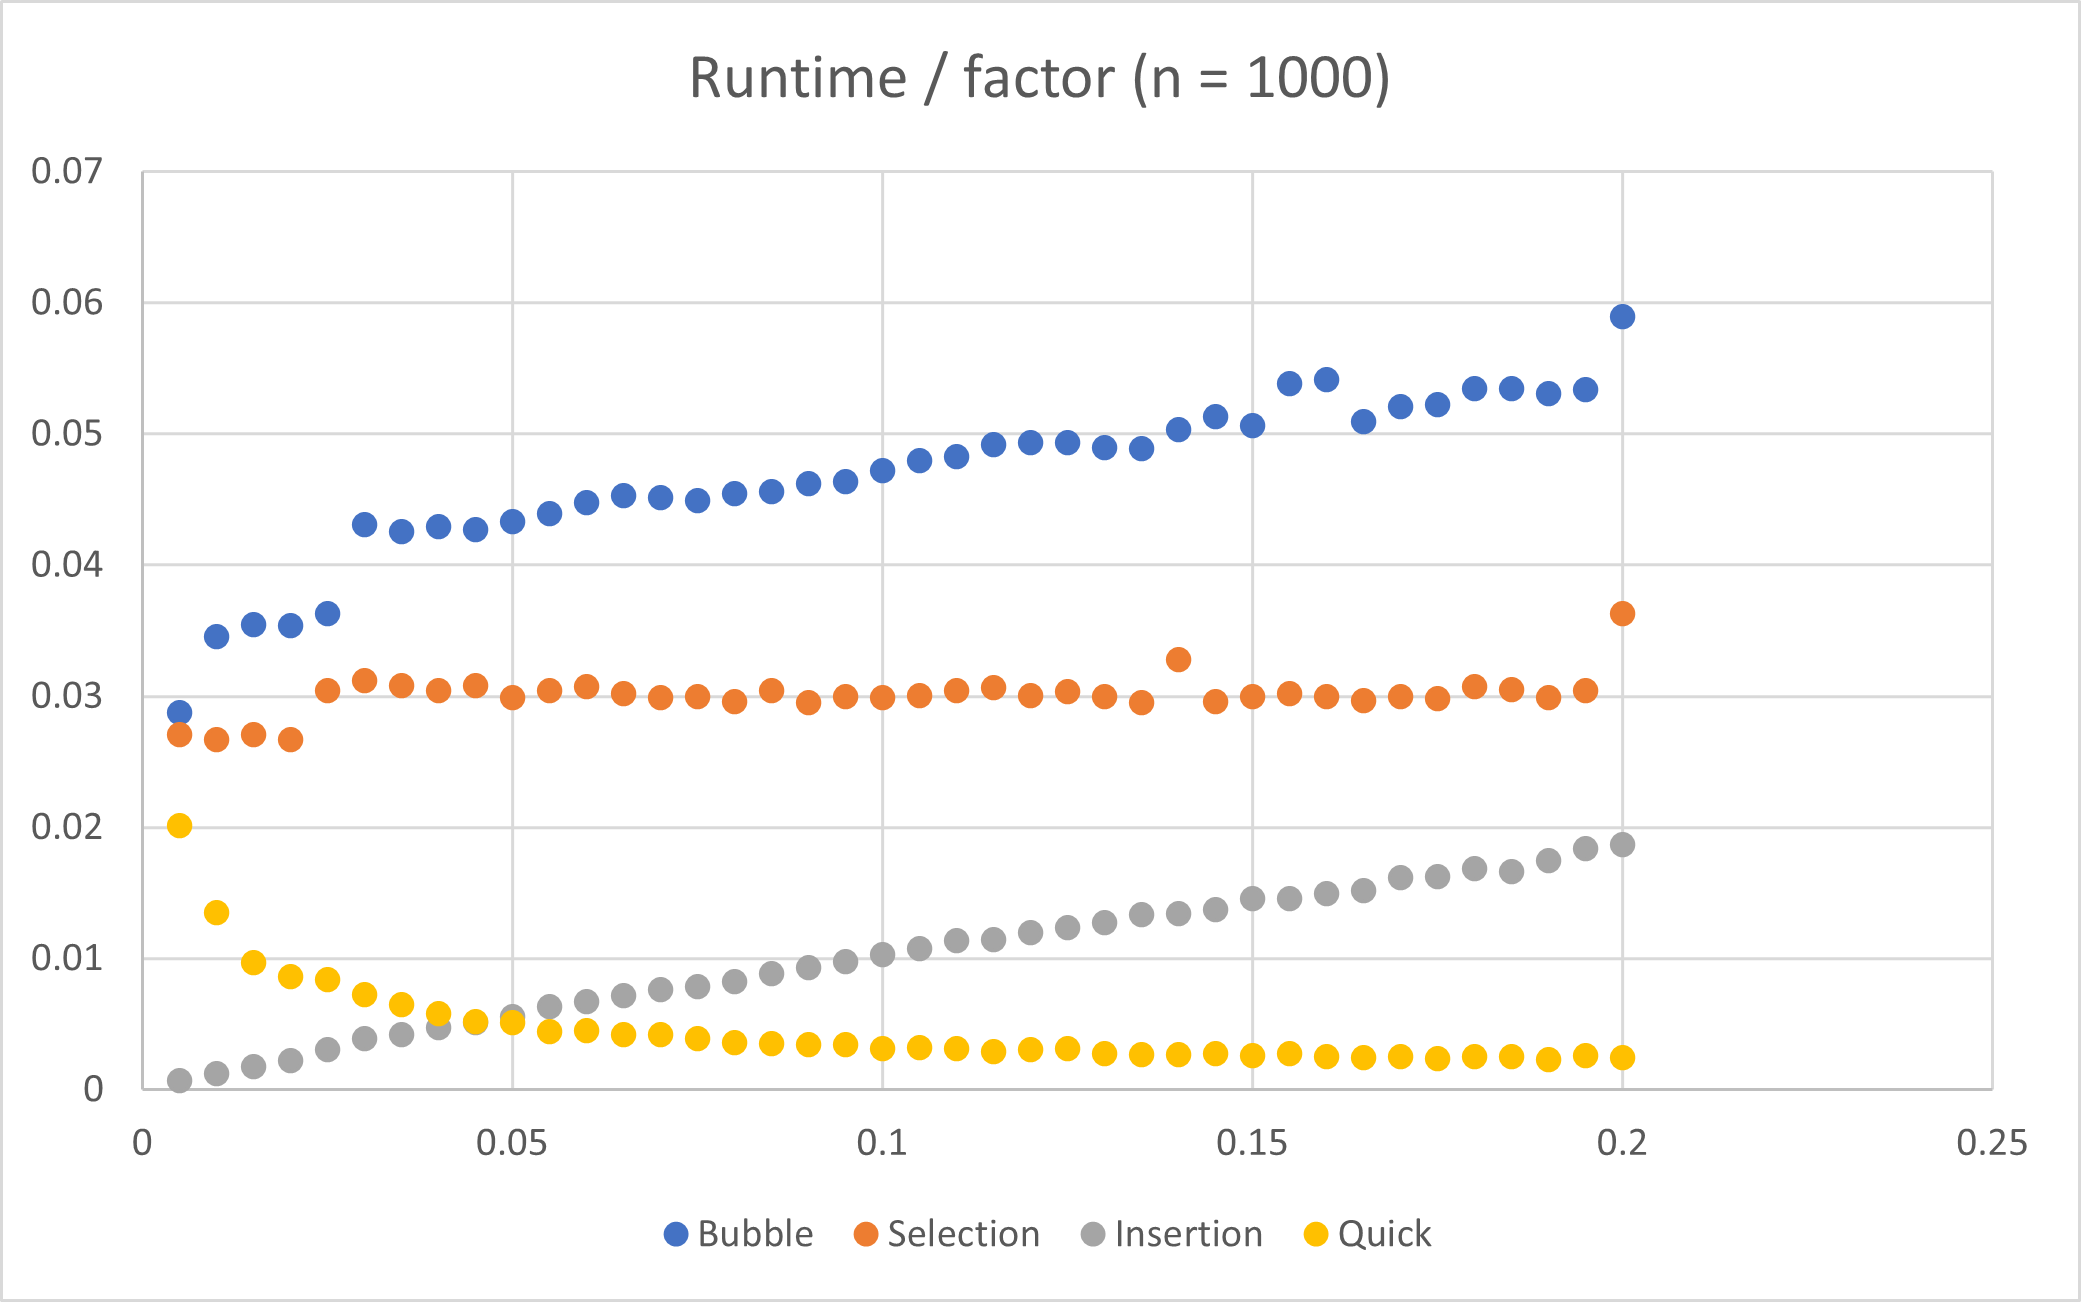
\includegraphics[width=0.49\textwidth]{Figures/sorted0005.png}\label{sorted0005}}
  \hfill
  \subfloat[$factor=0.005 \sim  0.2$, $n=100$]{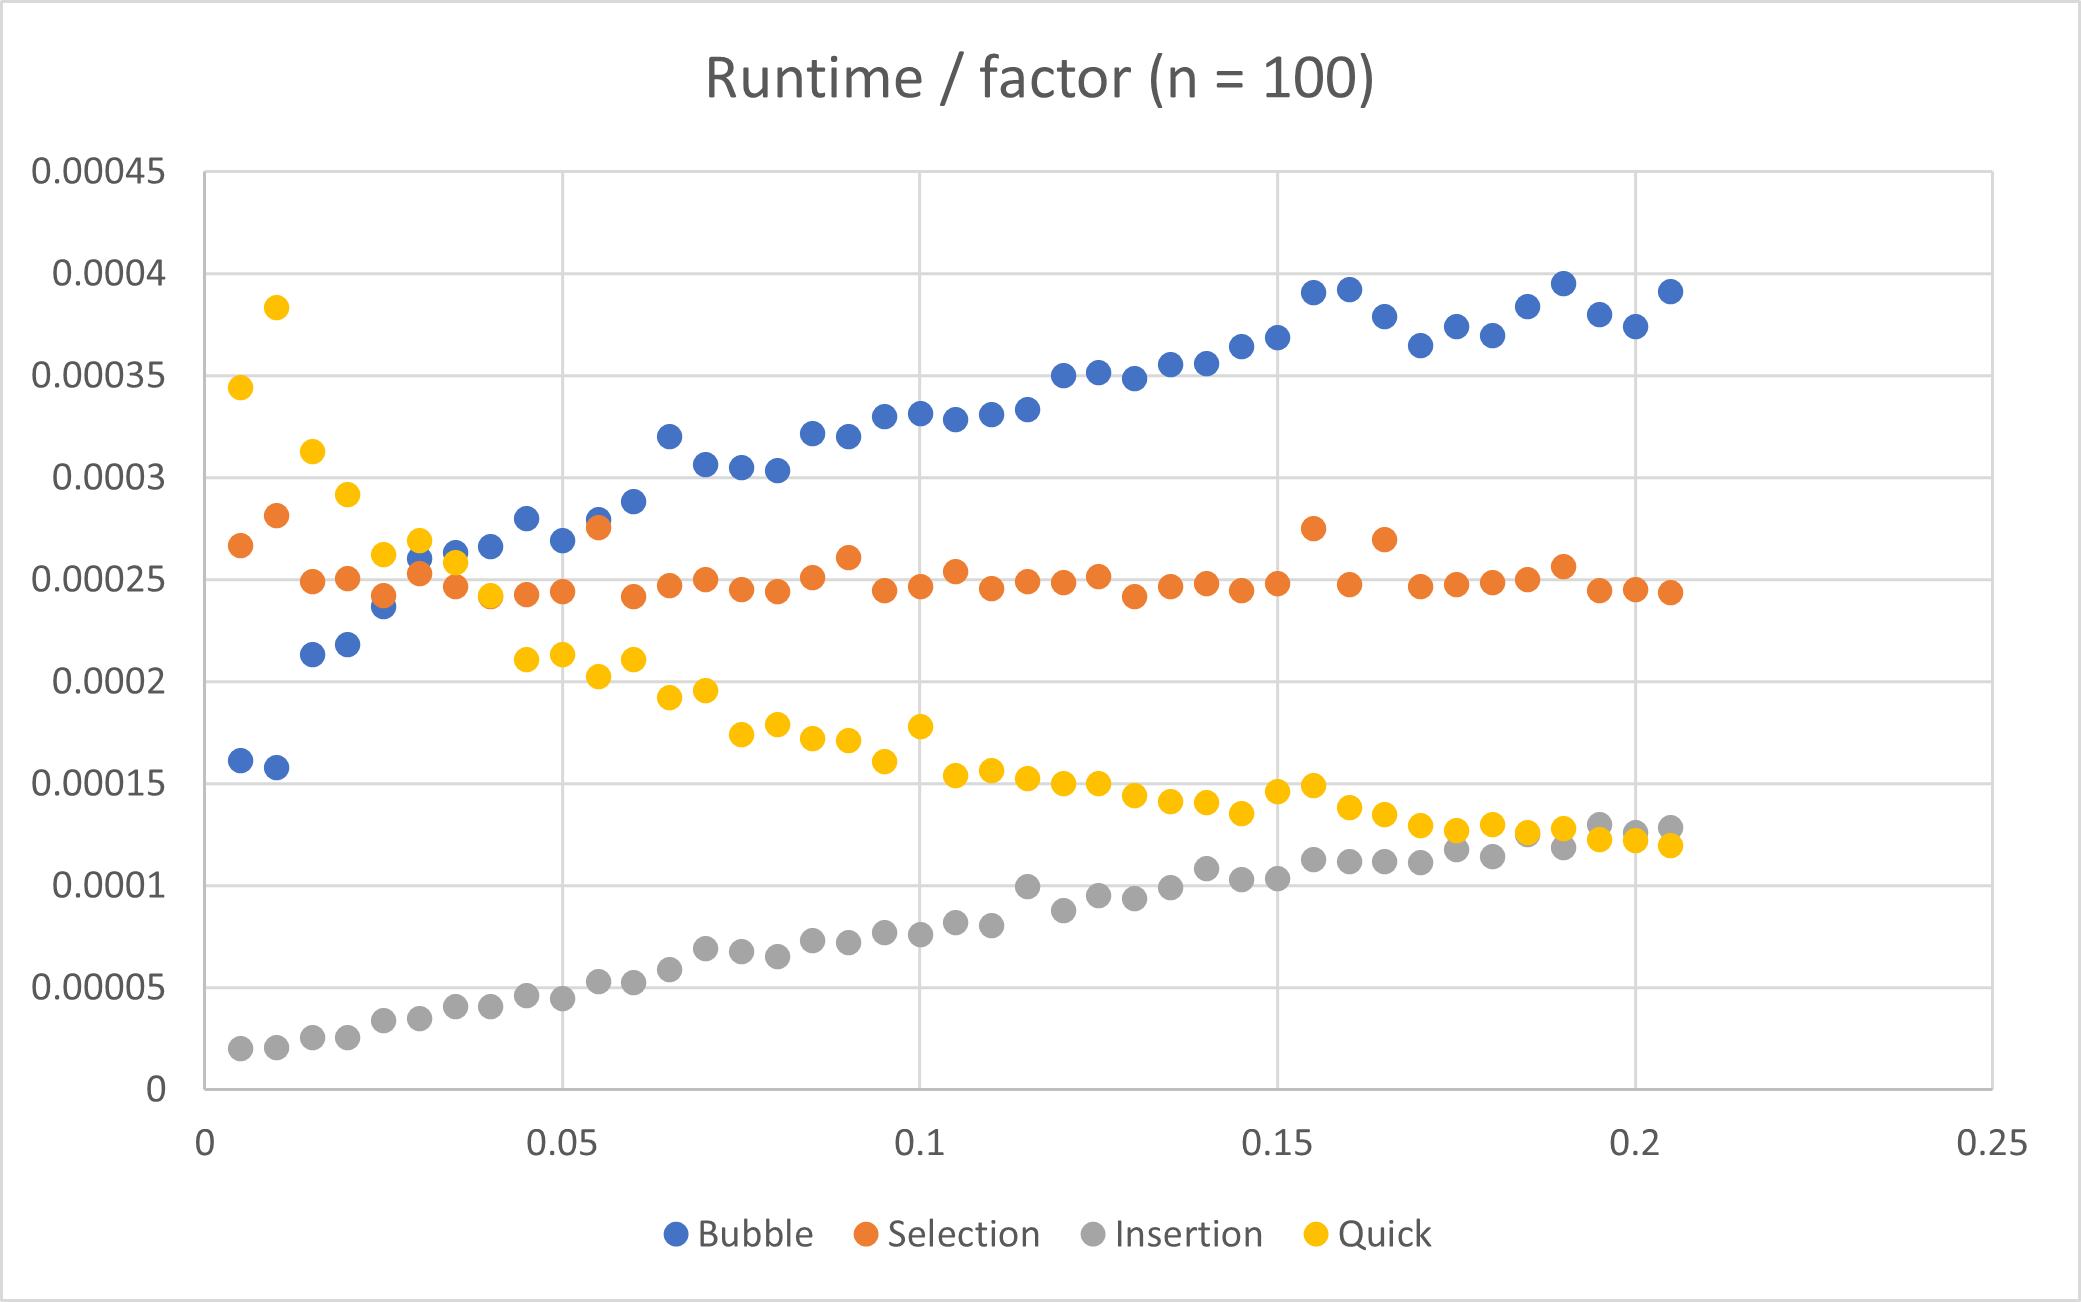
\includegraphics[width=0.49\textwidth]{Figures/sorted0005n100.png}\label{sorted0005n100}}
  \caption{Time complexities based on sorted factors}
\end{figure}

\bigskip

\begin{table}[htb!]
  \centering
  \begin{tabular}{ |p{3cm}||p{2cm}|p{2cm}|p{2cm}|  }
    \hline
    \multicolumn{4}{|c|}{\textbf{Time complexity}} \\
    \hline
    \textbf{Name} & \textbf{Best} & \textbf{Average} & \textbf{Worst} \\
    \hline 
    Bubble sort    & $n$     & $n^{2}$ & $n^{2}$ \\[0.5ex]
    Selection sort & $n^{2}$ & $n^{2}$ & $n^{2}$ \\[0.5ex]
    Insertion sort & $n$     & $nlogn$ & $nlogn$ \\[0.5ex]
    Quicksort      & $nlogn$ & $nlogn$ & $n^{2}$ \\[0.5ex]
    \hline
  \end{tabular}
  \caption{Sorting algorithms' time complexities}
  \label{time complexity}
\end{table}

\medskip

\section{Small Lists}
In this part, tests are set to evaluate the performance of quicksort in the cases of small lists.
\subsection{Quicksort performance under small lists}
In this section we tested sorting algorithms' performance under low values of n. 
We divided the test range into two. First n's range is $1 \sim 100$, and second range is $1 \sim 20$.
And we obtained the test result by running 500 and 5000 times per point respectively for
 the smooth graphs. Figure \ref{unsortedlow100}, \ref{unsortedlow20} show that the
performance of quicksort is worse than other elementary sorts under $n=7$. When the 
number of elements exceeds 20, quicksort shows better performance 
than the others. This is because when the number of elements is small, quicksort's 
recursion and copy parts are dominant factors to determine the time complexity.
But if the number exceeds a certain level, which is 20 in this test, 
the effectiveness of the algorithm begins to outperform structural shortcomings. 
 
\begin{figure}[hbt!]
  \centering
  \subfloat[$n=1 \sim 100$]{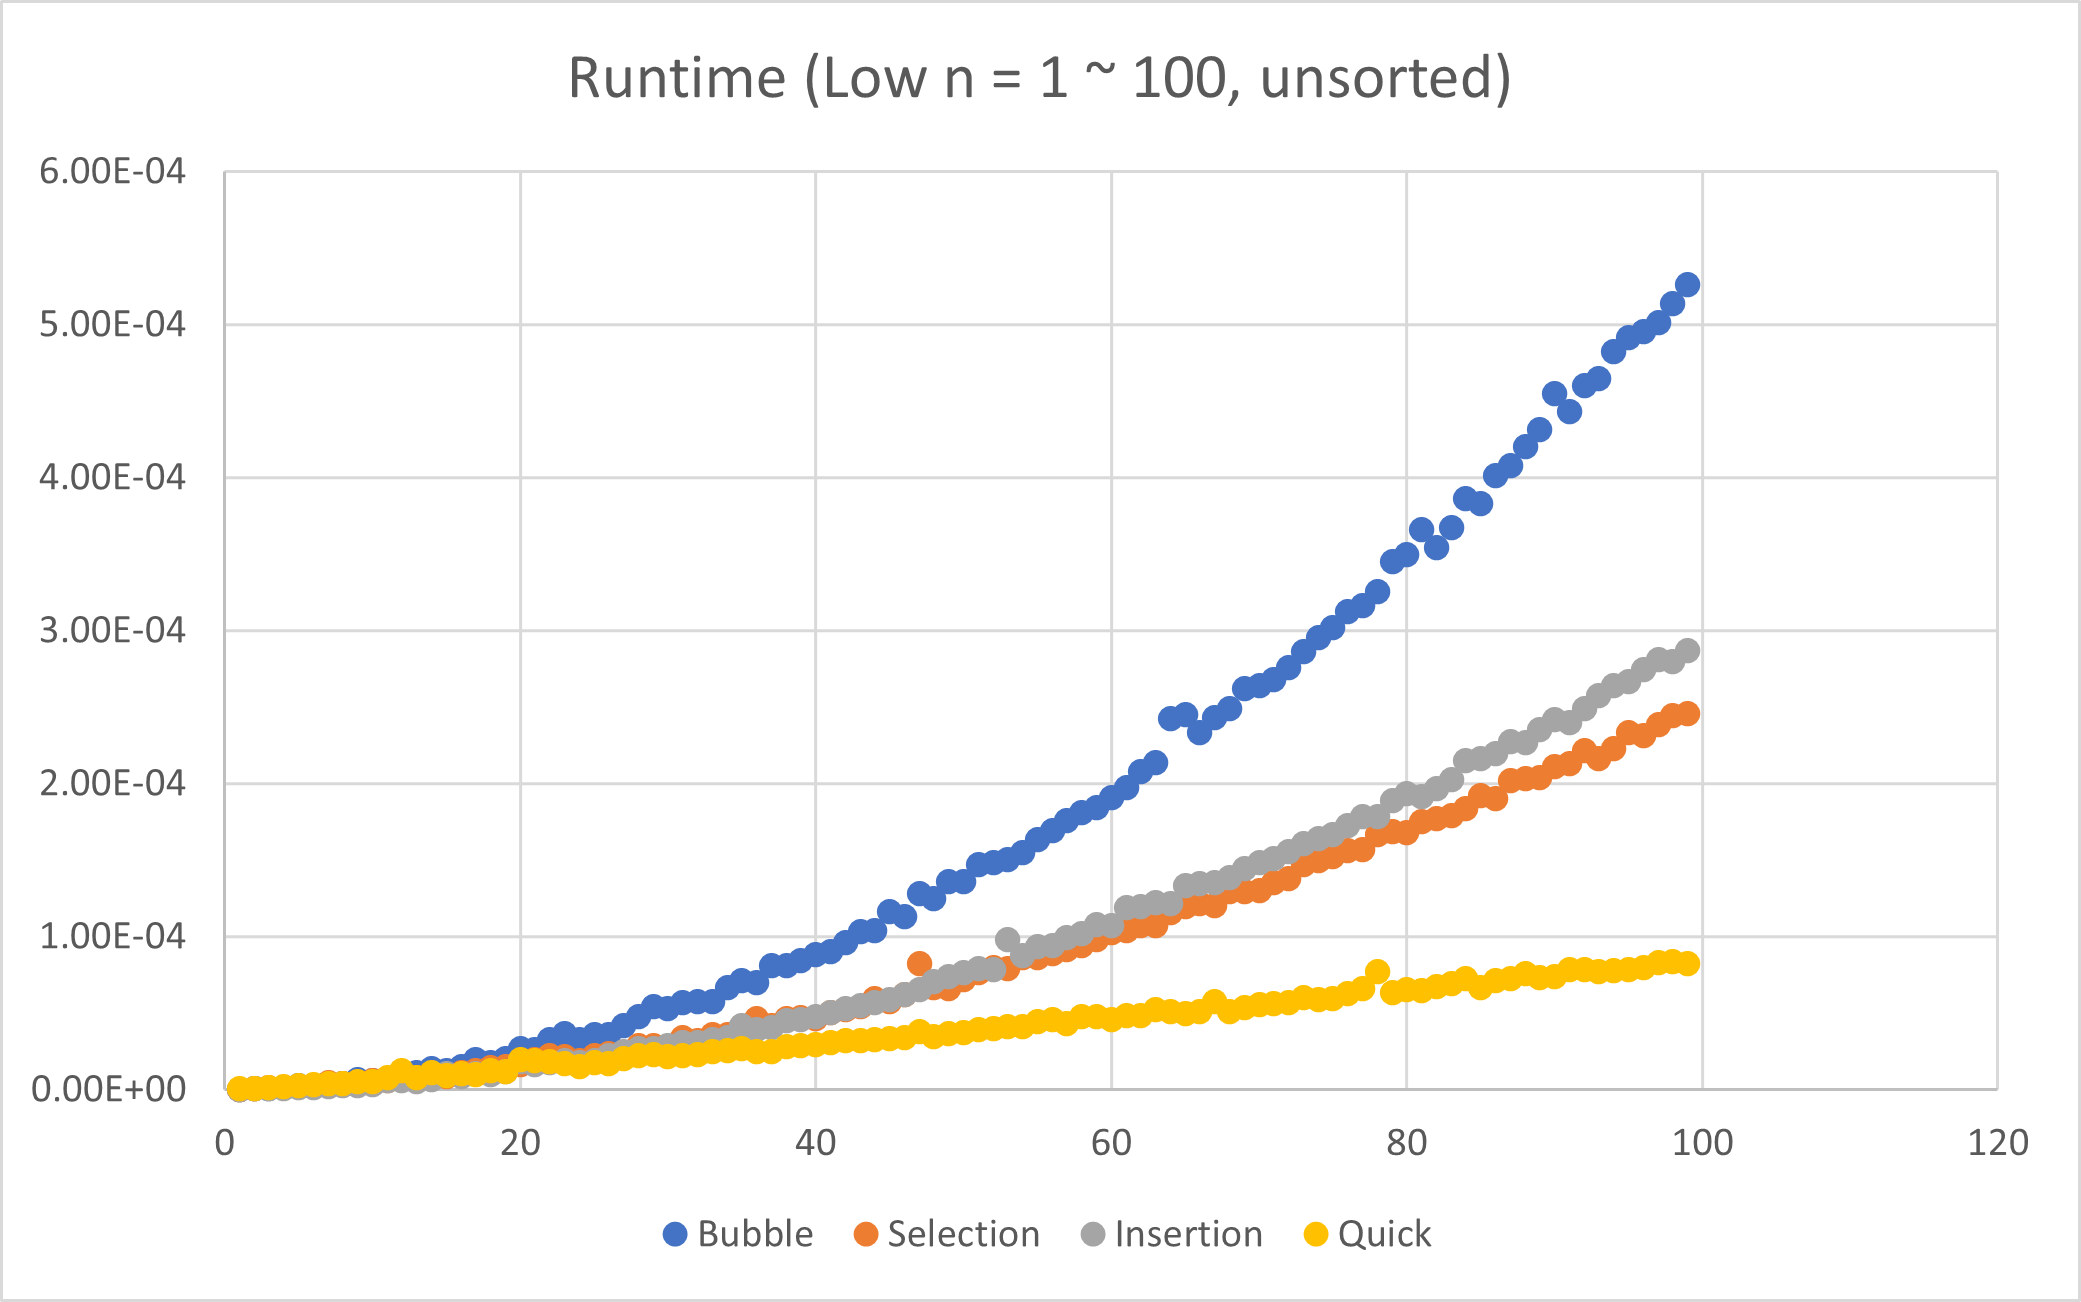
\includegraphics[width=0.49\textwidth]{Figures/unsortedlow100.png}\label{unsortedlow100}}
  \hfill
  \subfloat[$n=1 \sim 20$]{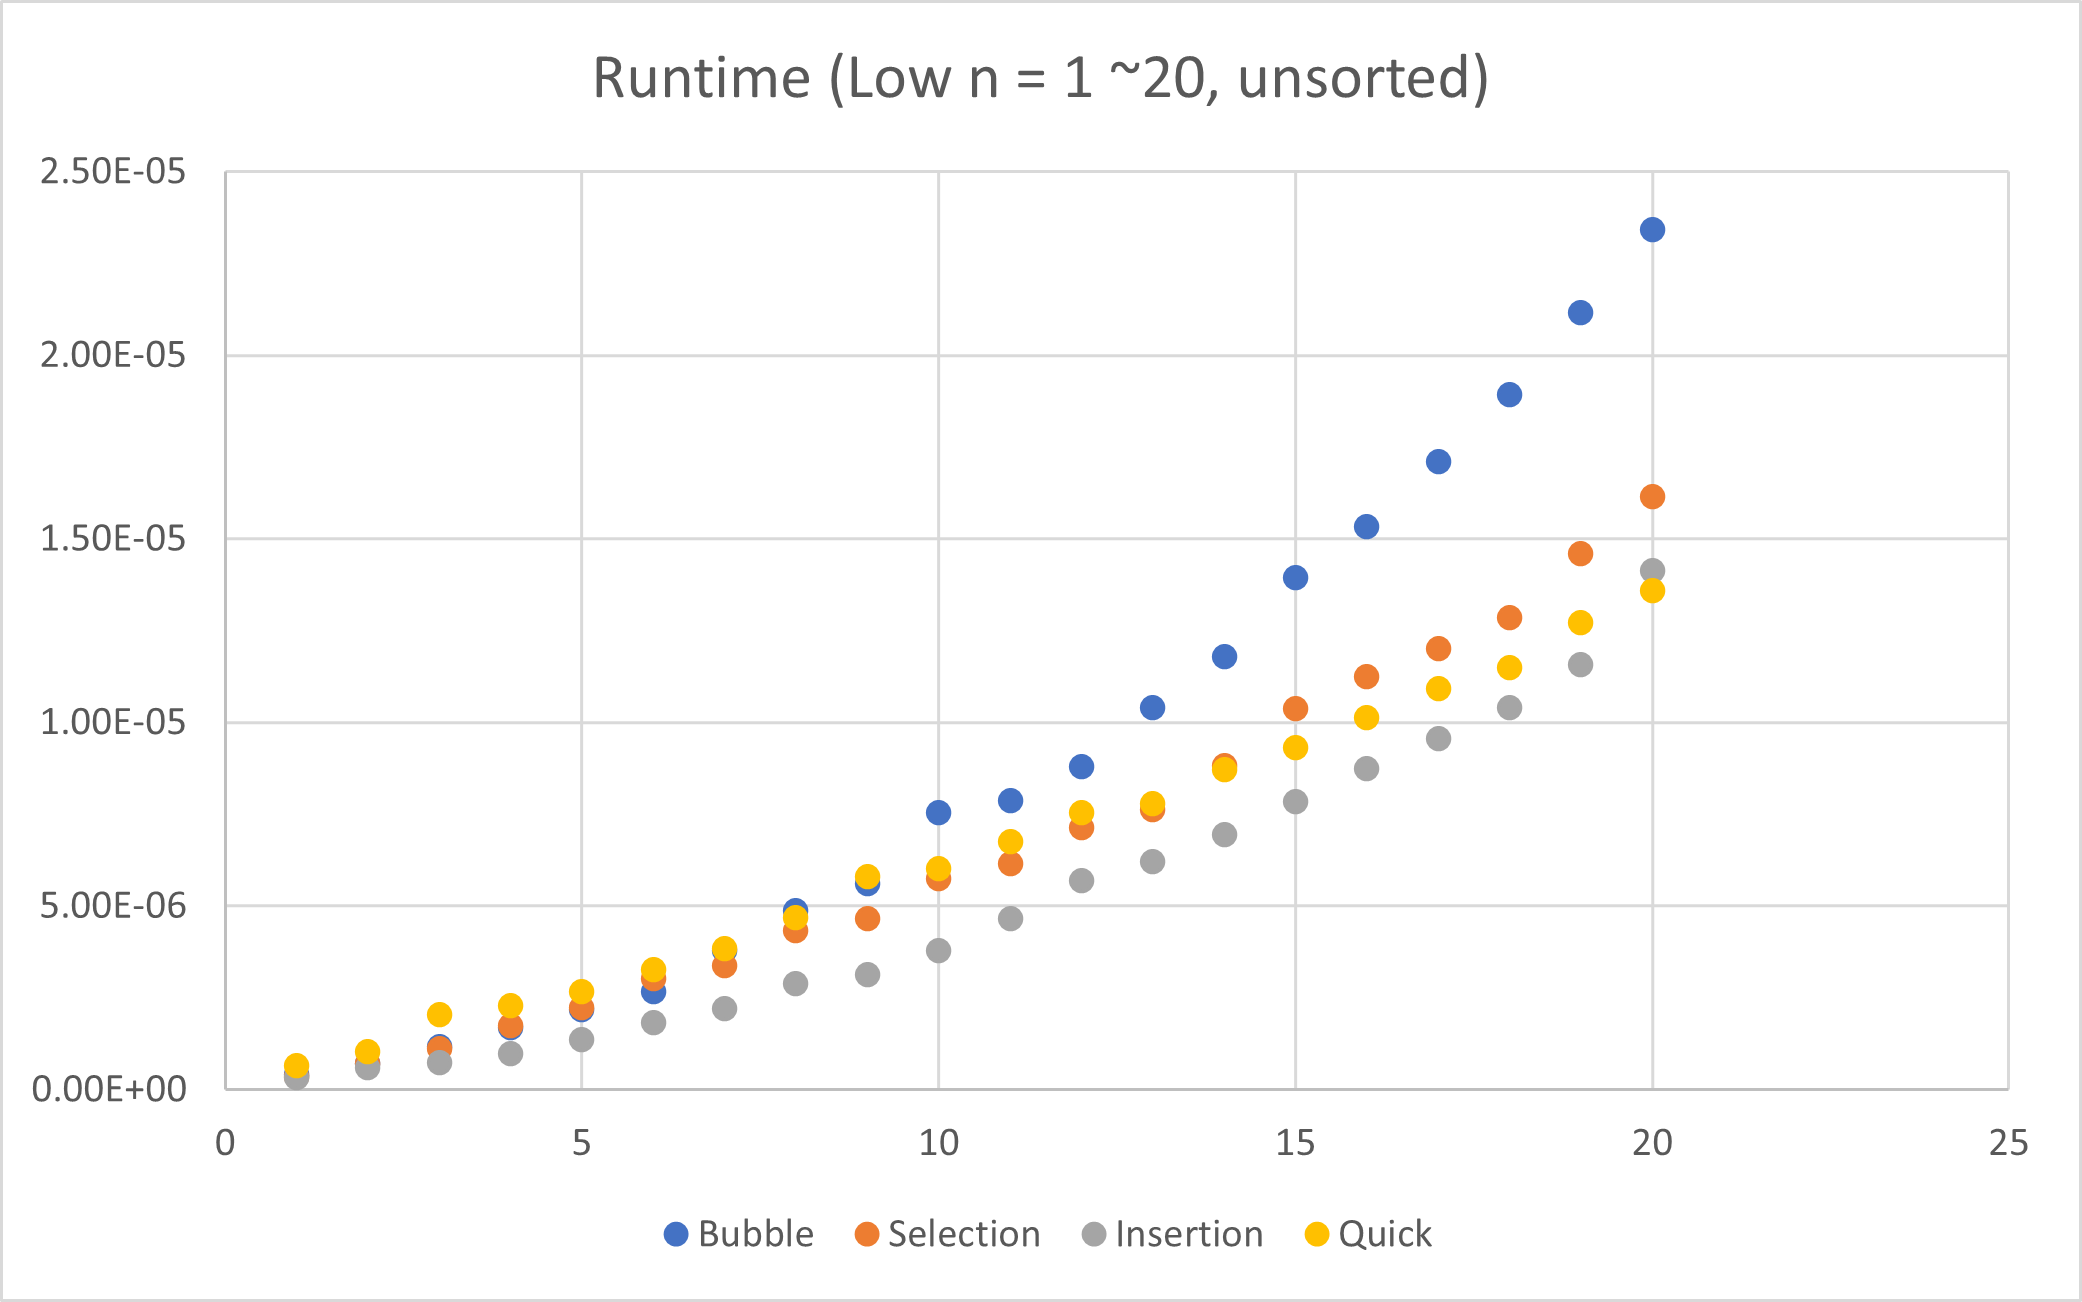
\includegraphics[width=0.49\textwidth]{Figures/unsortedlow20.png}\label{unsortedlow20}}
  \caption{Time complexities on small lists}
\end{figure}

\subsection{The best algorithm}
We thought about the best algorithm based on the test results. In order to get the 
best algorithm, we considered three factors, which are `1. type of algorithms'
, `2. number of elements', and `3. degree of alignment'. We consider these three 
factors one by one. 

~\newline\noindent First, `1. type of algorithms'. In terms of time complexity, quicksort and insertion 
sort are the best algorithms. But there are some factors that should be considered
to optimize the time complexity, which are `2. number of elements' and `3. degree of 
alignment'. Second, `2. number of elements'. When the number of
 elements are small, the diffierence of absoulute runtime among different 
 sorting algorithms is 
trivial. Except for a specific situation, which is using the sorting algorithm with
very few elements repeatedly, quicksort is the still best algorithm. If we can 
avoid the worst-case scenario, even though the length is small, quicksort's average
time complexity is $O(nlogn)$, which means clost to $n$. 
Third, `3. degree of alignment'. When a list is nearly sorted, quicksort algorithm's
effectiveness decreases significantly to $O(n^{2})$. In order to avoid the worst-case 
scenario, we modify the \verb|my_quicksort()| a little bit by choosing the
pivot with a middle element of the list and exchanging it with the first elemnt of 
the list. As quicksort is recursive function, 
if we choose the middle element in a sorted list, we can easily avoid the smallest 
or largest value in the list recursively. Figure \ref{finalsort1}, \ref{finalsort2} 
are the result of \verb|final_sort()|. 
Compared to the previous quicksort, they show clearly improved results in 
the worst case scenario.

\begin{figure}[hbt!]
  \centering
  \subfloat[$n=1000$, $factor=0.005 \sim 0.2$]{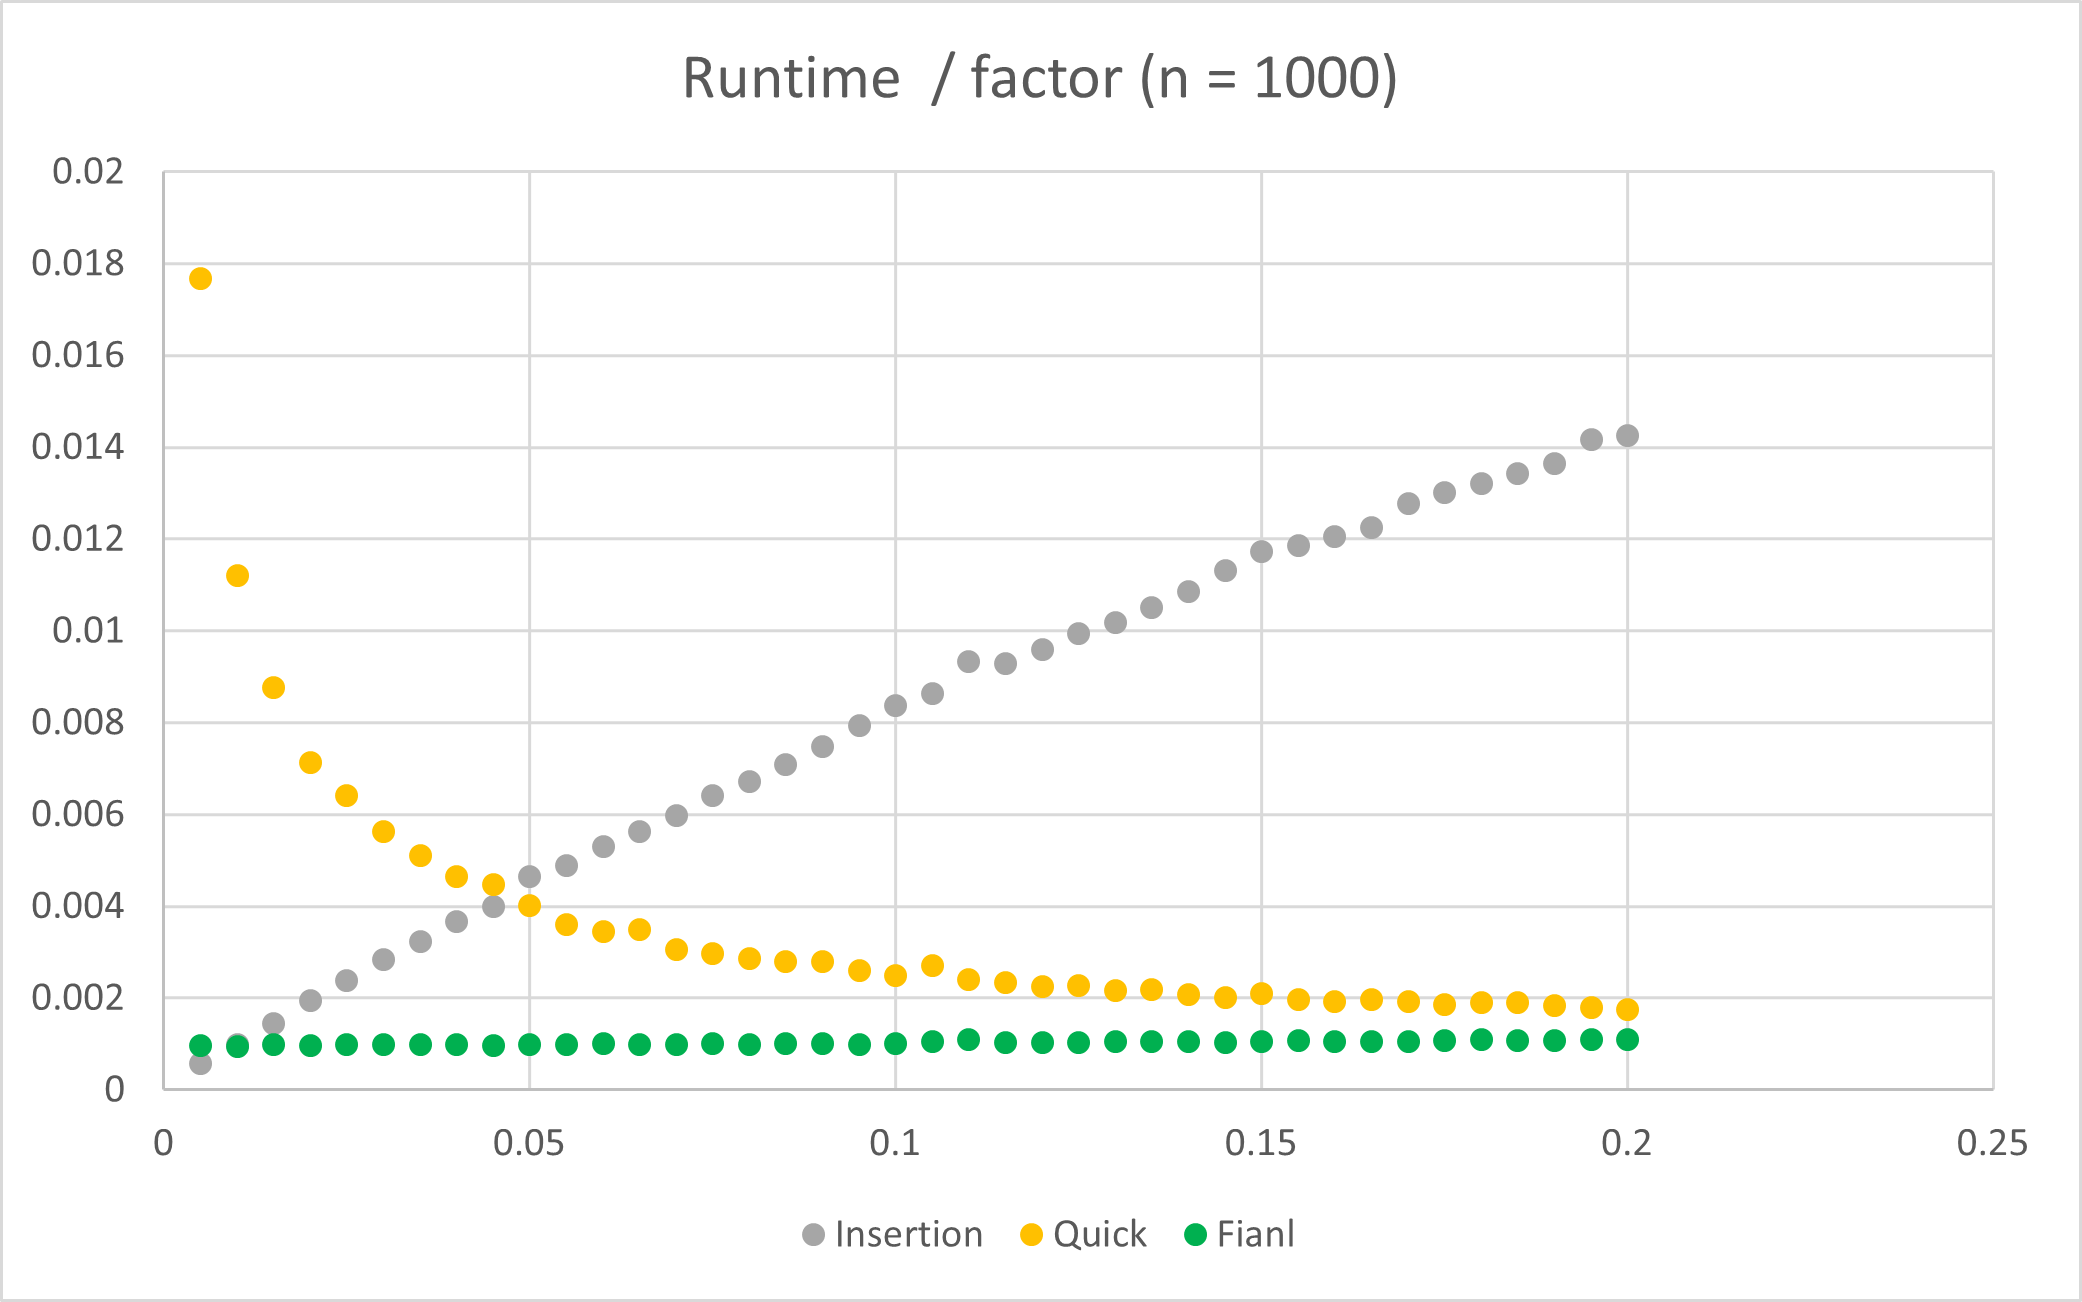
\includegraphics[width=0.49\textwidth]{Figures/finalsort1.png}\label{finalsort1}}
  \hfill
  \subfloat[$n=100$, $factor=0.005 \sim 0.2$]{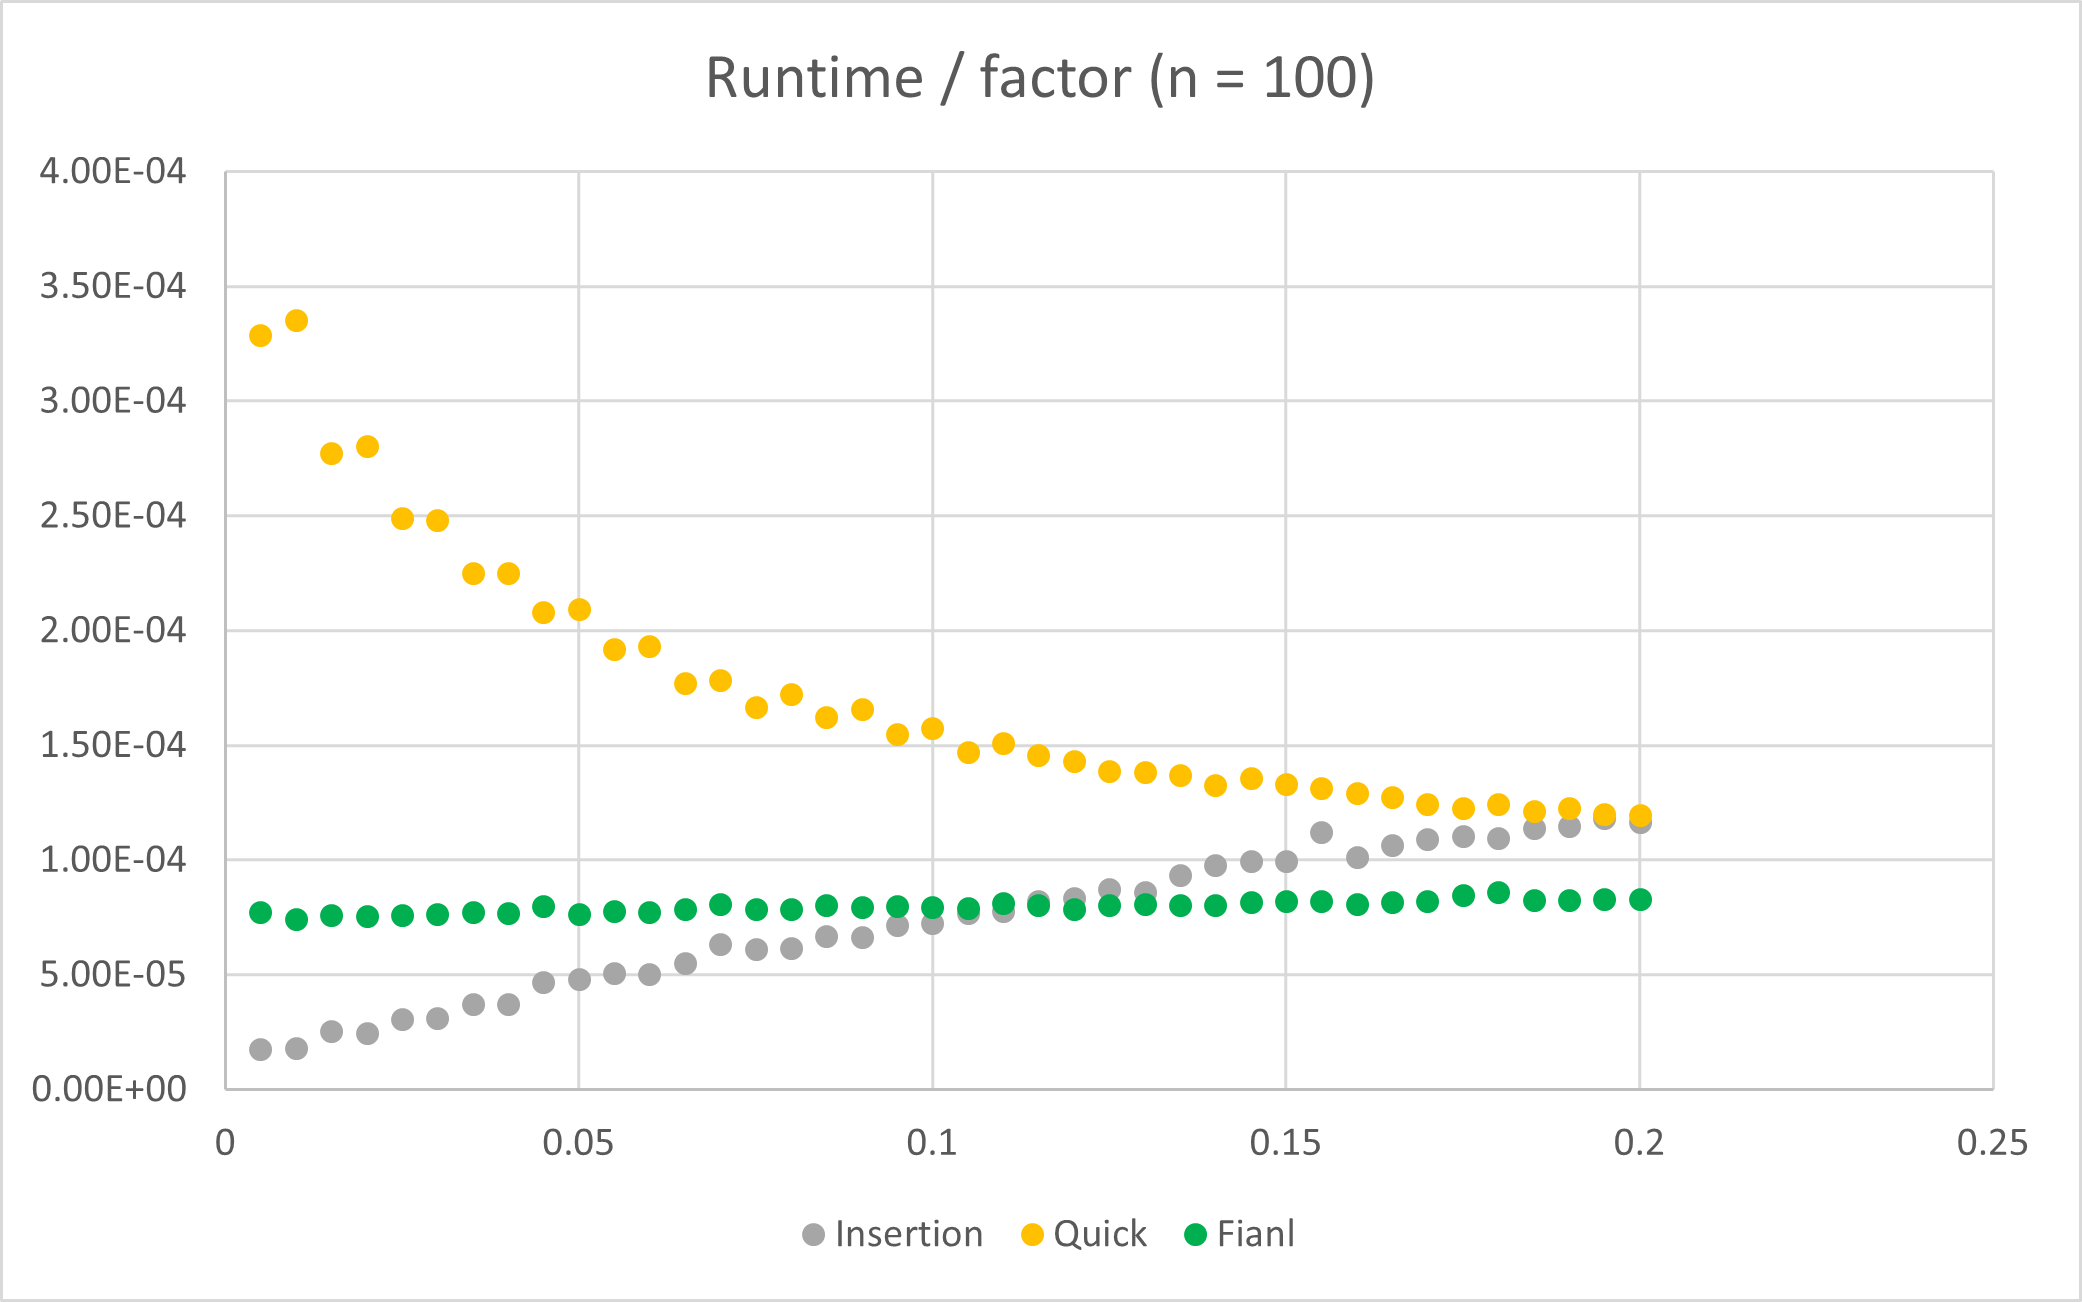
\includegraphics[width=0.49\textwidth]{Figures/finalsort2.png}\label{finalsort2}}
  \caption{Time complexity of improved quicksort}
\end{figure}
%finalsort1 factor 0.005 - 0.2, n 1000, 100times
%finalsort2 factor 0.005 - 0.2, n 100, 1000times

~\newline\noindent In order to improve a bit more, we combined quicksort with 
insertion sort. Based on the test result (Figure \ref{unsortedlow20}),
 when a list's length is less than equal 20, then we used insertion sort.
 As a result, \verb|fianl_sort()|'s runtime reduced to the insertion sort's runtime
 level when n is samll (Figure \ref{finalsort3n100}, \ref{finalsort3n20}).


 \begin{figure}[hbt!]
  \centering
  \subfloat[$n=100$, $factor=0.005 \sim 0.2$]{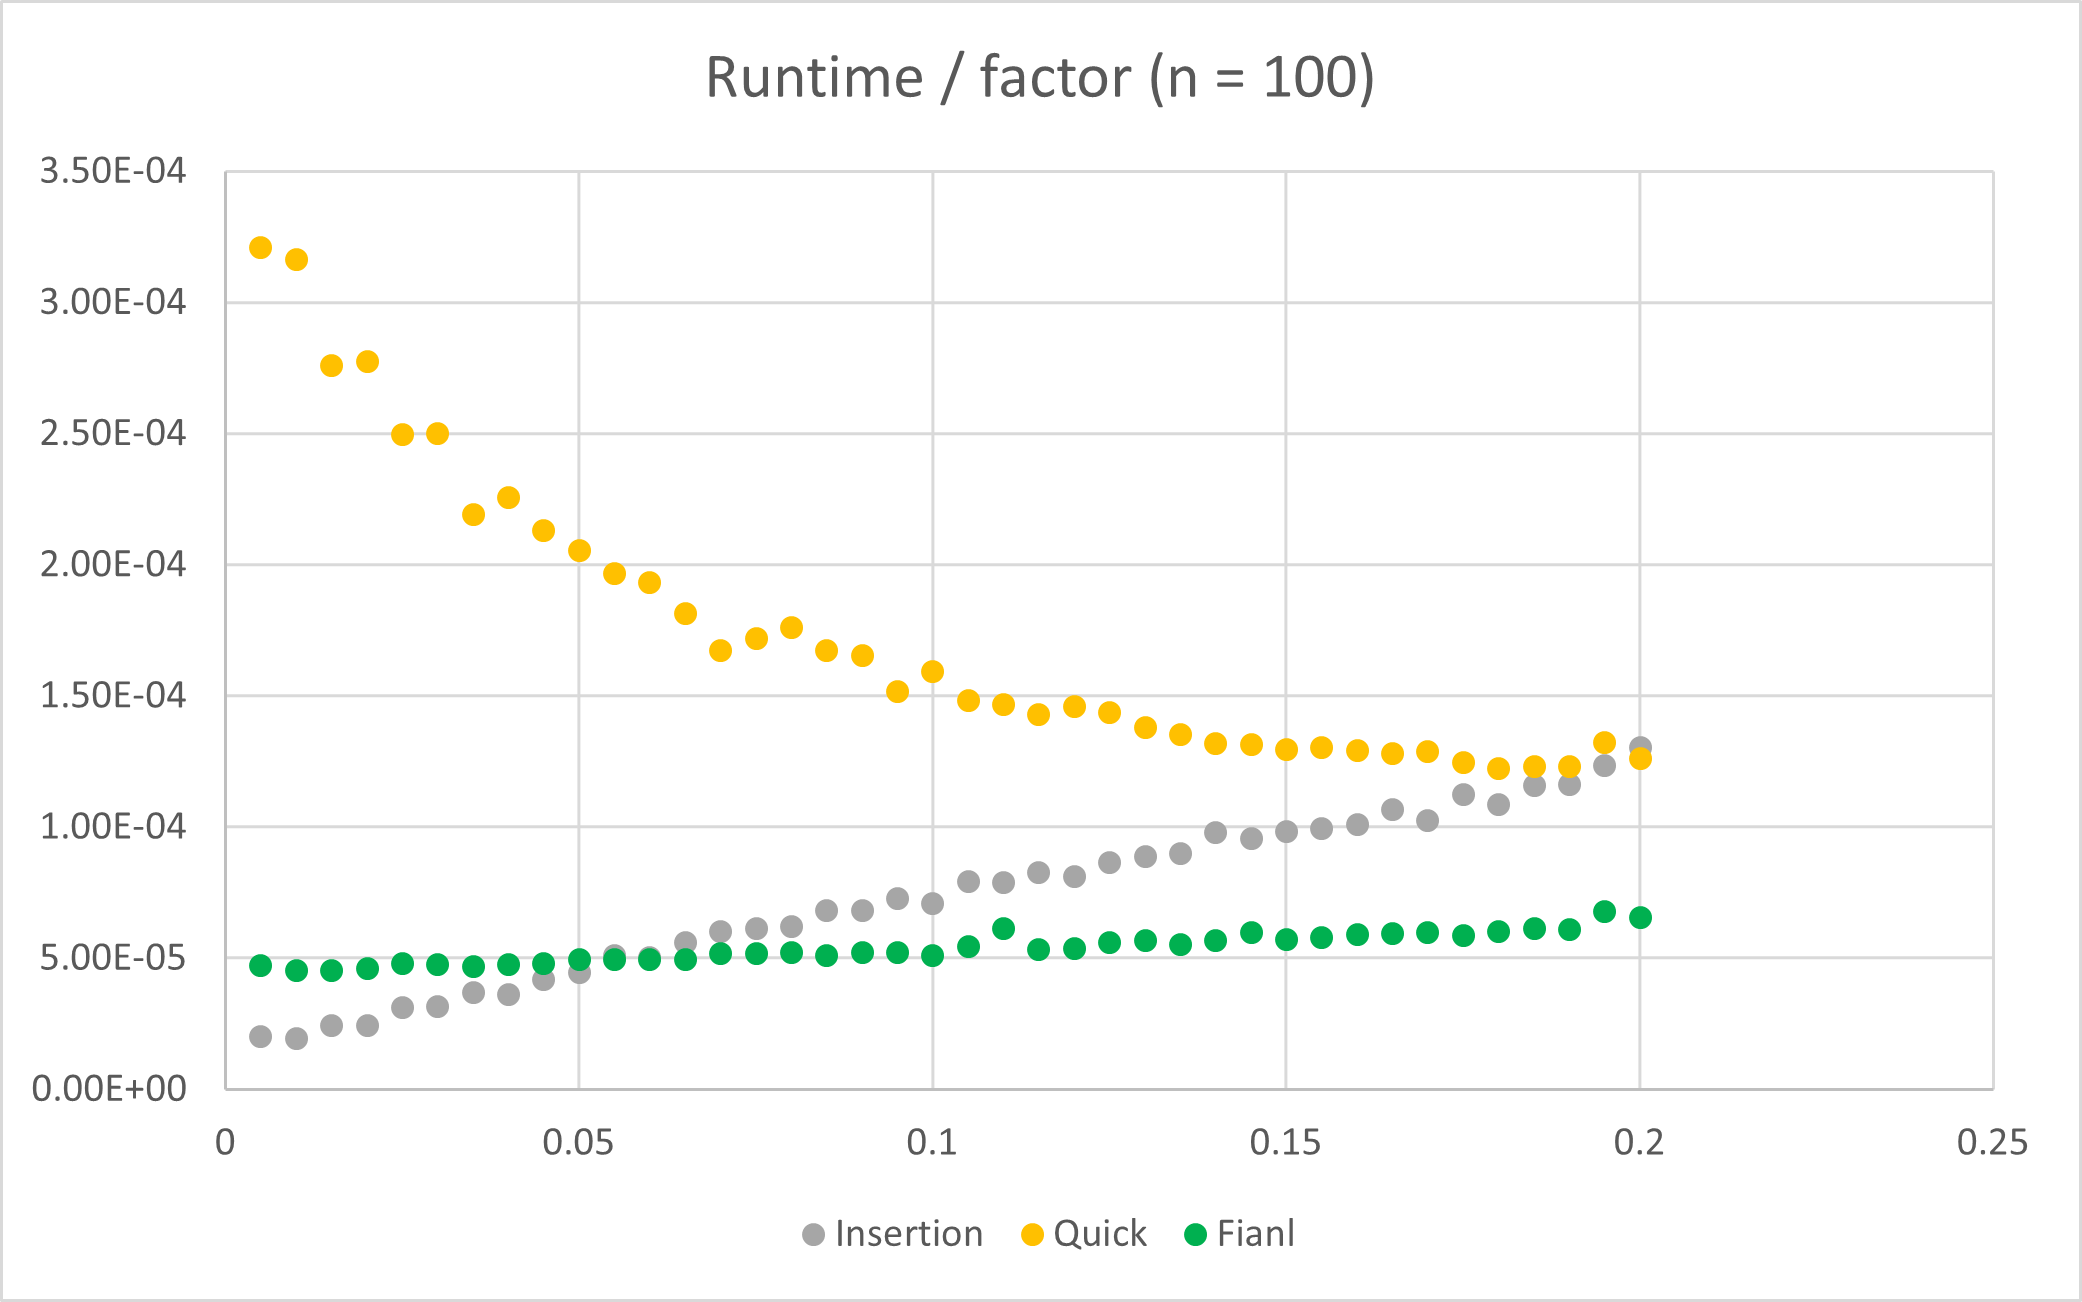
\includegraphics[width=0.49\textwidth]{Figures/finalsort3n100.png}\label{finalsort3n100}}
  \hfill
  \subfloat[$n=1 \sim 20$, unsorted]{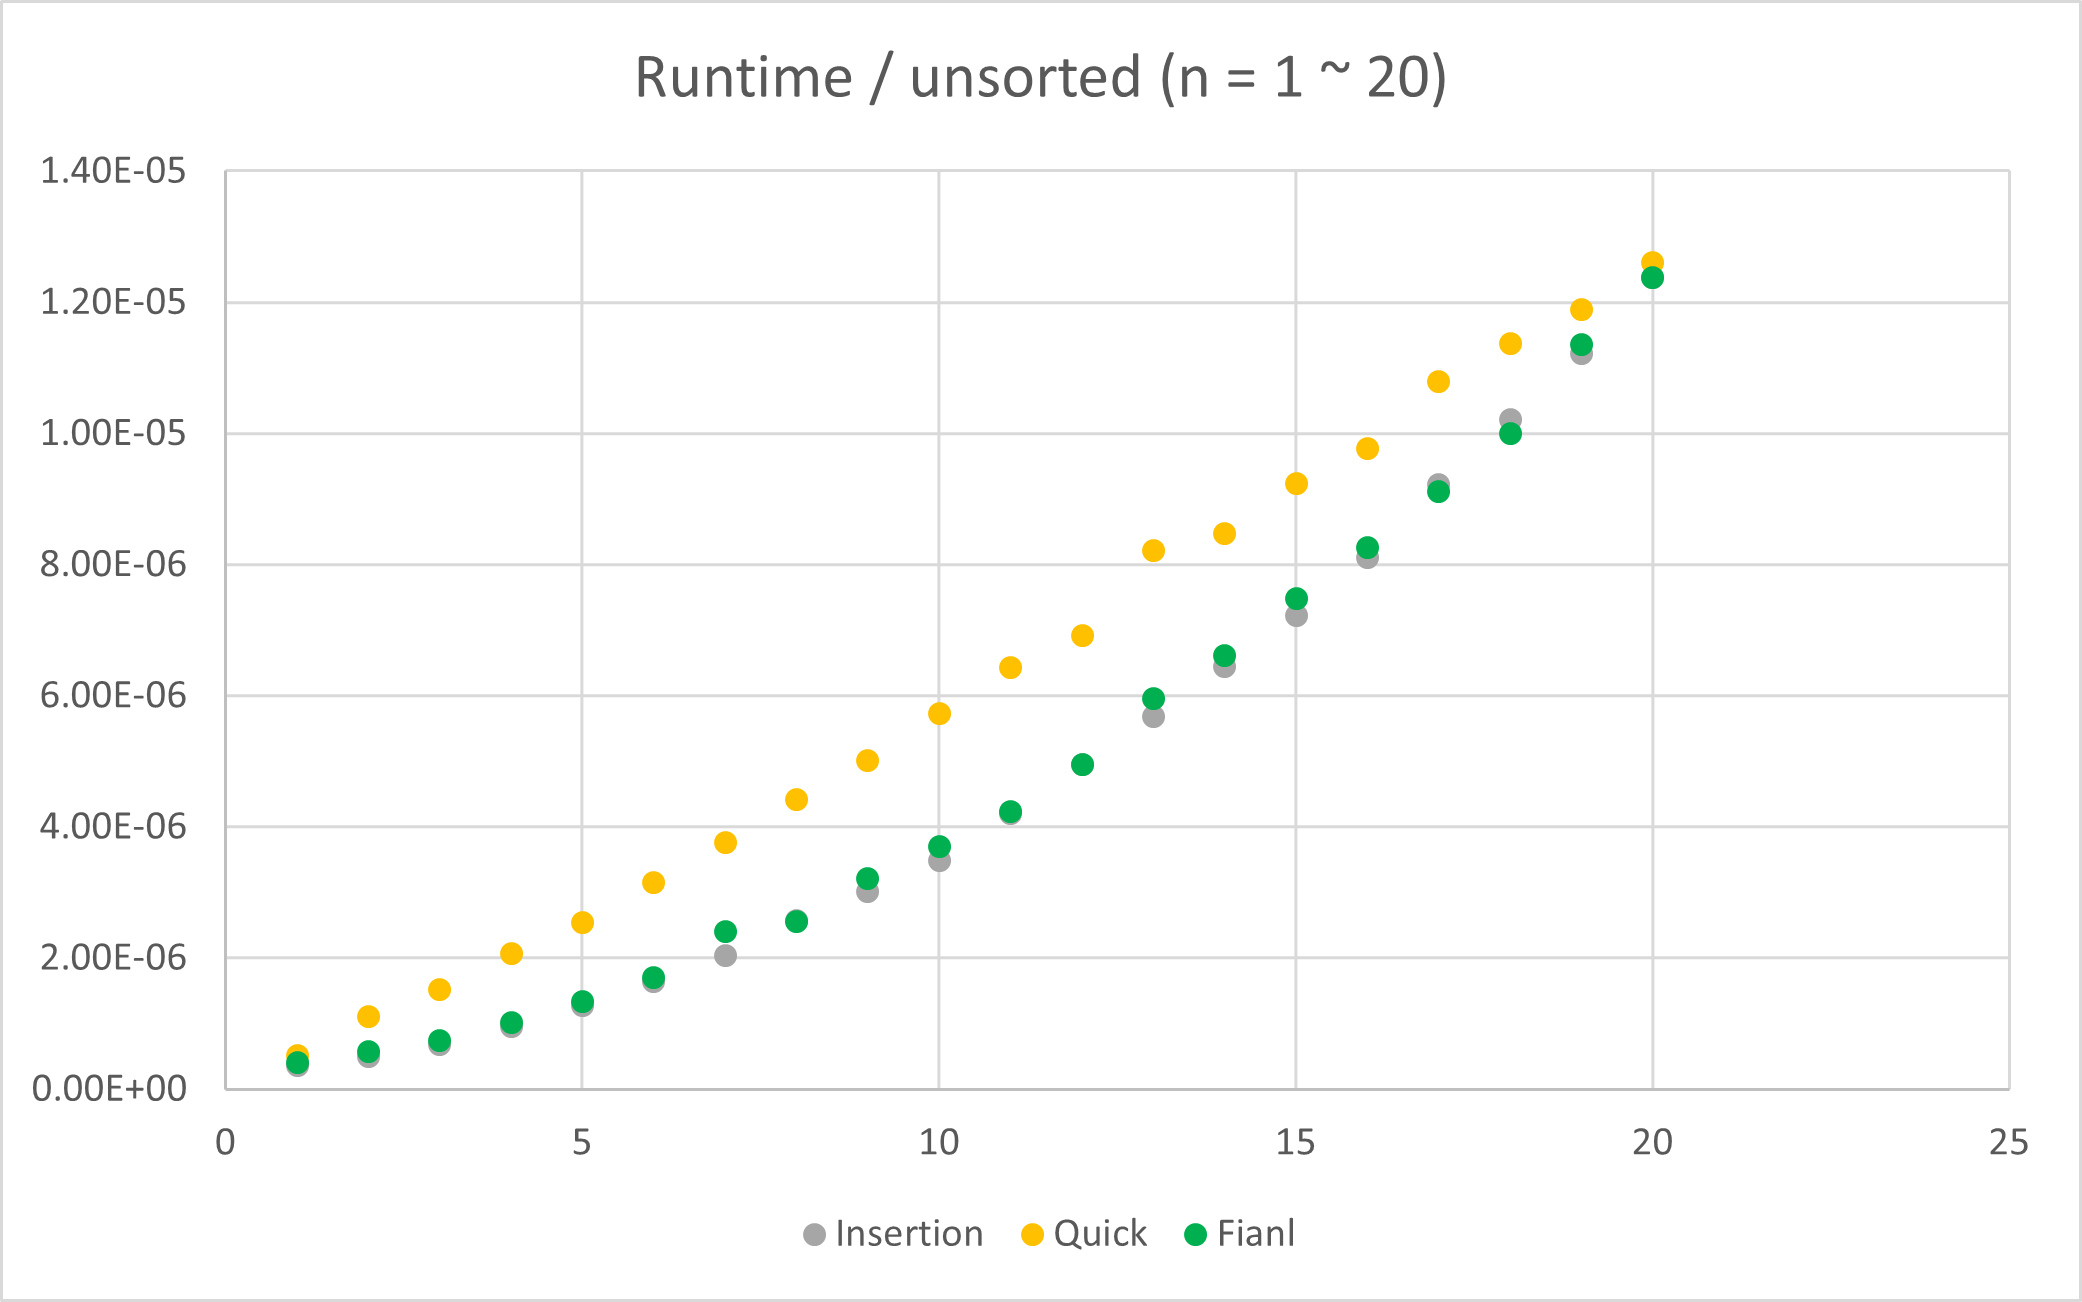
\includegraphics[width=0.49\textwidth]{Figures/finalsort3n20.png}\label{finalsort3n20}}
  \caption{Time complexity of final\_sort()}
\end{figure}

%finalsort3n100 factor 0.005 - 0.2, n 1000, 100times
%finalsort3n20 unsorted, n 100, 10000times

\newpage

\lstset{language=Python, basicstyle=\tiny, breaklines=true, showspaces=false,
  showstringspaces=false, breakatwhitespace=true, frame=single}
%\lstset{language=C,linewidth=.94\textwidth,xleftmargin=1.1cm}
\section*{Appendix: source code}
Below is all our test code for this lab.
\noindent \lstinputlisting{code.py}
\noindent \lstinputlisting{sorts.py}

\end{document}
